% gs -sDEVICE=pdfwrite -dCompatibilityLevel=1.5 -dNOPAUSE -dQUIET -dBATCH -dPrinted=false -sOutputFile=note.pdf _note.pdf

% openany: remove blank pages.
% oneside: remove the page alternation
\documentclass[a4paper,10pt,openany,oneside]{memoir}
\usepackage[italian]{babel}
\usepackage[utf8]{inputenc}
\usepackage{graphicx} % immagini
\usepackage{xurl}  % ritorno a capo nelle URL
\usepackage{hyperref} % stile dei link
\hypersetup{
  colorlinks   = true,    % Colours links instead of ugly boxes
  urlcolor     = blue,    % Colour for external hyperlinks
  linkcolor    = black,   % Colour of internal links
  citecolor    = red      % Colour of citations
}

\usepackage[lining]{ebgaramond}
\usepackage[scaled=0.8]{courierten}

% Remove "Chapter" from the chapter name
\usepackage[center]{titlesec}
\titleformat{\chapter}{\LARGE\centering}{\thechapter}{5pt}{}
% % Reduce the gap around the chapter title
\titlespacing*{\chapter}{0pt}{0pt}{20pt}
\setcounter{tocdepth}{4}

% hide section numbering
\makeatletter
\renewcommand{\@seccntformat}[1]{}
\makeatother

% hide chapter numbering
\titleformat{\chapter}
  {\Large\centering} % format
  {}                % label
  {0pt}             % sep
  {\huge}           % before-code

\pagestyle{plain}

%%%%%%%%%%%%%%%%%%%%%%%%%%%%%%%%%%%%%%%%%%%%%%%%%%%%%%%%%%%%%%%%%%%%%%%%%%%%

\begin{document}

\author{Zan Wenjie}  % 昝文杰
\date{\tiny\textit{Accumulate negli anni - Redatte dal 2023}}
\title{\vspace*{-0.5cm}\huge\textit{Note per} \\ \HUGE\textit{Il cacciatore} \\ \vspace*{0.3em} \huge\textit{(e racconti)} \hfill\\ \hfill\\ \hfill\\ 
\includegraphics[scale=0.25, trim={60cm 70cm 260cm 55cm}, clip]  {USGS-PlanetMars-TopographicalMap.png} } % trim={left bottom right top}

\maketitle
\thispagestyle{empty}

\newpage
\tableofcontents*
\newpage


\chapter{Titano}

\section{Luminosità del cielo}

L'alta atmosfera di Titano è opaca alla luce visibile. Ergo il cielo di Titano è costantemente coperto da nuvole spesse e la luminosità, anche durante il giorno, è simile a quella di un temporale o al chiuso, in casa. Vedi la GIF per la simulazione generata dall'articolo che cito sotto.

"Sky brightness and viewing conditions are expected to be quite different from Earth and Mars due to Titan's farther distance from the Sun (~10 AU) and complex haze layers in its atmosphere. The sky brightness model videos show what a typical sunny day may look like standing on the surface of Titan based on radiative transfer models.

For astronauts who see with visible light, the daytime sky has a distinctly dark orange color and appears uniform in all directions due to significant Mie scattering from the many high-altitude haze layers. The daytime sky is calculated to be ~100-1000 times dimmer than an afternoon on Earth, which is similar to the viewing conditions of a thick smog or dense fire smoke. The sunsets on Titan are expected to be "underwhelming events", where the Sun disappears about half-way up in the sky (~50° above the horizon) with no distinct change in color. After that, the sky will slowly darken until it reaches night. However, the surface is expected to remain as bright as the full Moon up to 1 Earth day after sunset."

\url{https://iopscience.iop.org/article/10.3847/1538-3881/aae519} Titan's Twilight and Sunset Solar Illumination, Jason W. Barnes et al. 2018

"Outdoor light levels were much higher (11,080–18,176 lux) than indoors (112–156 lux). The higher lux levels protective of myopia (>1000 lux) were measured at the tree shade (5556–7876 lux) and with hat (4112–8156 lux). [...]  illuminance levels reaching 130,000 lux on a clear day to 15,000 lux under shaded or cloudy conditions." (\url{https://www.ncbi.nlm.nih.gov/pmc/articles/PMC6656201/}, "The Effects of Different Outdoor Environments, Sunglasses and Hats on Light Levels: Implications for Myopia Prevention", Carla Lanca) Quindi ci sono due ordini di grandezza tra la luce in casa e quella all'esterno. Titano quindi è più scuro che al chiuso.


"In visible light, Saturn will make the sky on Titan's Saturn-facing side appear slightly brighter, similar to an overcast night with a full moon on Earth. Saturn's rings are hidden from view owing to the alignment of Titan's orbital plane and the plane of the rings. Saturn is expected to show phases, akin to the phases of Venus on Earth, that partially illuminate the surface of Titan at night, except for eclipses."

\url{https://books.google.pt/books?id=xyNRygEACAAJ&redir_esc=y} Saturn's Moon Titan: From 4. 5 Billion Years Ago to the Present - an Insight Into the Workings and Exploration of the Most Earth-Like World in the Outer Solar System, Ralph Lorenz


\includegraphics[scale=0.6, trim={0 0 0 19cm}, clip]{Visible_and_Infrared_Sunsets_on_Titan.png}

Colore del cielo al tramonto, simulazione (vedi gif corrispondente nei files).


\includegraphics[scale=0.6]{Huygens_surface_color.jpeg}

L'unica immagine di Titano esistente al momento. "Real color".

\url{https://photojournal.jpl.nasa.gov/catalog/PIA07232}

This image was returned yesterday, January 14, 2005, by the European Space Agency's Huygens probe during its successful descent to land on Titan. This is the colored view, following processing to add reflection spectra data, and gives a better indication of the actual color of the surface. Initially thought to be rocks or ice blocks, they are more pebble-sized. The two rock-like objects just below the middle of the image are about 15 centimeters (about 6 inches) (left) and 4 centimeters (about 1.5 inches) (center) across respectively, at a distance of about 85 centimeters (about 33 inches) from Huygens. The surface is darker than originally expected, consisting of a mixture of water and hydrocarbon ice. There is also evidence of erosion at the base of these objects, indicating possible fluvial activity.


\section{Laghi}

\includegraphics[scale=0.14]{PIA20021-ligeia-mare.jpg}

I laghi di Titano: Ligeia Mare (solo perchè belle foto del Kraken non le ho trovate)

\url{https://photojournal.jpl.nasa.gov/catalog/PIA20021}


These images from the Radar instrument aboard NASA's Cassini spacecraft show the evolution of a transient feature in the large hydrocarbon sea named Ligeia Mare on Saturn's moon Titan.

Analysis by Cassini scientists indicates that the bright features, informally known as the "magic island," are a phenomenon that changes over time. They conclude that the brightening is due to either waves, solids at or beneath the surface or bubbles, with waves thought to be the most likely explanation. They think tides, sea level and seafloor changes are unlikely to be responsible for the brightening.

The images in the column at left show the same region of Ligeia Mare as seen by Cassini's radar during flybys in (from top to bottom) 2007, 2013, 2014 and 2015.

The bottom image was acquired by Cassini on Jan. 11, 2015, and adds another snapshot in time as Cassini continues to monitor the ephemeral feature (previously highlighted in PIA18430). The feature is apparent in the images from 2013 and 2014, but it is not present in other images of the region.

Cassini has observed similar transient features elsewhere in Ligeia Mare, and also in Kraken Mare (see PIA19047). These features are the first instances of active processes in Titan's lakes and seas to be confirmed by multiple detections. Their changing nature demonstrates that Titan's seas are not stagnant, but rather, dynamic environments.

The Cassini radar team plans to re-observe this particular region of Ligeia Mare one more time during Cassini's final close flyby of Titan in April 2017. The results may further illuminate the phenomenon responsible for the appearance of the transient features.

The large image panel shows Ligeia Mare in its entirety. Ligeia is Titan's second-largest liquid hydrocarbon sea, and has a total area of about 50,000 square miles (130,000 square kilometers), making it 50 percent larger than Lake Superior on Earth. This panel is a mosaic of five synthetic aperture radar images acquired by Cassini between 2007 and 2014. It shows a region approximately 330 by 305 miles (530 by 490 kilometers) in area.

[...] The images have been colorized and processed for aesthetic appeal.


\section{Clima e precipitazioni}

"Titan's surface temperature is about 94 K (-179.2C). At this temperature, water ice has an extremely low vapor pressure, so the little water vapor present appears limited to the stratosphere. Titan receives about 1\% as much sunlight as Earth. Before sunlight reaches the surface, about 90\% has been absorbed by the thick atmosphere, leaving only 0.1\% of the amount of light Earth receives."

Ci sono decisamente nuvole, precipitazioni, etc con un ciclo del metano identico al ciclo dell'acqua terrestre. Però non è mai chiaro cosa si vede in luce visibile e cosa in infrarossi.

GIF delle nuvole sopra Ligeia nelle note: \url{https://photojournal.jpl.nasa.gov/catalog/PIA18420}

"This animated sequence of Cassini images shows methane clouds moving above the large methane sea on Saturn's moon Titan known as Ligeia Mare.

The spacecraft captured the views between July 20 and July 22, 2014, as it departed Titan following a flyby. Cassini tracked the system of clouds as it developed and dissipated over Ligeia Mare during this two-day period. Measurements of the cloud motions indicate wind speeds of around 7 to 10 miles per hour (3 to 4.5 meters per second).

The timing between exposures in the sequence varies. In particular, there is a 17.5-hour jump between the second and third frames. Most other frames are separated by one to two hours.

A separate view, PIA18421, shows the location of these clouds relative to features in Titan's north polar region."

Ci sono decisamente tempeste di "sabbia" su Titano: Observational evidence for active dust storms on
Titan at equinox, S. Rodriguez et al, 2018

\section{Magnetosfera}

"Titan spends 95\% of its time within Saturn's magnetosphere, which may help shield it from the solar wind." Dato che "Titan orbits Saturn once every 15 days and 22 hours.", il 5\% del proprio periodo dovrebbe essere il tempo che spende al di fuori della magnetosfera, ovvero (0.05 * 16 * 24) = 19h ogni due settimane.

\section{Atmosfera}

Gli strati esterni sono di un blu intenso, quelli interni giallo-arancio per via delle toline. 

\includegraphics*{Titan-haze-layer.jpg}

\url{https://www.flickr.com/photos/kevinmgill/50320802233/in/photostream/}

Titan - November 19 2007

Processed using calibrated red, green, and blue filtered images of Titan taken by Cassini on November 19 2007. NASA/JPL-Caltech/SSI/CICLOPS/Kevin M. Gill

\hfill 

\includegraphics*{Titan_-_June_18_2014-haze-true-color.png}

\url{https://www.flickr.com/photos/kevinmgill/50343380682/in/photostream/}

Titan - June 18 2014

Processed using calibrated red, green, blue, and ultraviolet filtered images taken by Cassini on June 18 2014. \textbf{The blue image is only used on a small part to colorize the star at the top left. The rest of the image uses UV in the blue channel}. [...] NASA/JPL-Caltech/SSI/CICLOPS/Kevin M. Gill


\section{Quadrangoli: St-09 Belet e St-01 Ligeia}
I quadrangoli di Titano non sono ancora stati definiti.

La nomenclatura "St" si può estrapolare dalle line gioviane e saturniane mappate ad oggi, per esempio Europa Je, Ganimede Jg, Encelado Se... Titano quindi dovrebbe essere St.

Riguardo alla posizione del quadrangoli, ho sovrapposto la definizione "standard" a 15 quadrangoli delle lune gioviane (e altri pianetini) trovata qui: \url{https://ntrs.nasa.gov/api/citations/19930001644/downloads/19930001644.pdf} alla mappa delle principali features di albedo note ad oggi, trovata qui: \url{https://solarsystem.nasa.gov/resources/17492/map-of-titan-with-labeled-features/}.

Si ottiene che il polo Nord è ovviamente St-01, mentre l'Adiri è spezzato in due dai quadrangoli St-09 e  St-08. Date le coordinate di George, però siamo di certo in St-09 (288-216, -22-22).

Riguardo ai nomi, St-08 contiene principalmente la feature scura Belet, St-09 è occupato soprattutto dallo Shangri-la, ma St-01 contiene tre mari: Kraken, Ligeia, e Punga. Kraken è il più grande ma esce dal quadrangolo (tecnicamente il centro è a 68 N, quando St-01 finisce a 66 N), quindi prendo Ligeia.

Risultato:
\begin{itemize}
\item St-01 Ligeia: 180-65N, 0-360 E 
\item St-08 Belet: 22N-22S, 288-216E
\item St-09 Shangri-la: 22N-22S, 216-144E
\end{itemize}

Altre note sui quadrangoli di lune varie:

\begin{itemize}
  \item Quadrangoli di Europa: Je 
  \begin{itemize}
    \item \url{https://solarviews.com/eng/eurmap.htm}
    \item \url{https://www.researchgate.net/publication/234039235_Geologic_mapping_of_Europa}
  \end{itemize}
  \item Quadrangoli di Cerere: Ac 
  \item Quadrangoli di Ganimede: Jg
  \item Quadrangoli di Enceladus: Se 
  \begin{itemize}
    \item \url{https://commons.wikimedia.org/wiki/File:Enceladus_quadrangles_PIA08419.png} 
    \item \url{https://www.jpl.nasa.gov/images/pia08419-the-enceladus-atlas} 
    \item \url{https://citeseerx.ist.psu.edu/document?repid=rep1&type=pdf&doi=067a5b1137804054705cacd66a3dfd4b652e56cd}
  \end{itemize}
  \item Indizio del processo di creazione dei quadrangoli: \url{https://www.researchgate.net/publication/331289249_Planetary_Mapping_A_Historical_Overview}
  \item Fonte: Batson, R.M., in Planetary Cartography, 261–276, 1990.
\end{itemize}


\includegraphics[scale=0.07, angle=90]{PIA20713-Titan-SaturnMoon-LabeledFeaturesIAU-June2015.jpg}

Mappa di Titano, annotata (infrarossi)

\url{https://photojournal.jpl.nasa.gov/catalog/PIA20713}


\includegraphics[scale=0.08]{PIA19657-SaturnMoon-Titan-NorthPole-20140407.jpeg}

\includegraphics[scale=0.08]{PIA19657-SaturnMoon-Titan-SouthPole-20140407.jpeg}

Mappa dei poli di Titano, annotata (infrarossi)

\section{Saturno nel cielo di Titano}

Esempio dal simulatore della NASA \url{https://space.jpl.nasa.gov/}, apertura 90°:

\includegraphics[scale=0.4]{saturn-from-titan-90deg-angle.jpeg}



\chapter{Cerere}

Di Cerere dico pochissimo, per cui non servono troppe info e Wikipedia in genere è sufficiente.

Per immagini, vedi missione Dawn: \url{https://solarsystem.nasa.gov/missions/dawn/galleries/images}

NASA Trek: \url{https://trek.nasa.gov/ceres} (disponibile anche per altri corpi celesti)




\chapter{Marte}

Vedi i libri nella repo, specialmente l'atlante e "The Atmosphere and Climate of Mars" per un sacco di info interessanti sulle nuvole e sul vento.

\section{Livelli di radiazioni al suolo}

Marte è seriamente radioattivo.

Assumendo in modo grezzo 1 Gy = 1 Sv (che potrebbe quasi avere senso dato che si parla di background radiation), un anno su Marte raggiunge già livelli di radioattività chiaramente legati a un aumento del rischio di sviluppare tumori.

\begin{itemize}
  \item Dose minima annuale chiaramente correlata a un aumento del rischio di cancro: 100mSv.
  \begin{itemize}
    \item Altra reference dopo un po' di ricerca per sicurezza: \url{https://dceg.cancer.gov/news-events/news/2020/low-dose-monograph}, dove "low dose" è definito come $<100$mG (interessante come usa Gy invece di Sv, il che aiuta un sacco)
    \item M. Hauptmann et al., Epidemiological Studies of Low-Dose Ionizing Radiation and Cancer: Summary Bias Assessment and Meta-Analysis, JNCI Monographs, Volume 2020, Issue 56, July 2020, Pages 188–200, \url{https://doi.org/10.1093/jncimonographs/lgaa010}
  \end{itemize}
  \item Radioattività di fondo di Marte: $\sim$0.3mG al giorno, varia da 0.2 a 0.6 durante le aurore (\url{https://mars.nasa.gov/news/large-solar-storm-sparks-global-aurora-and-doubles-radiation-levels-on-the-martian-surface/}).
  \item Secondo Wikipedia, la surface equivalent dose rate è di \textbf{27 uSv/h}, quindi 27 uSv/h * 24h = 648 uSv/g = \textbf{0.65 mSv/g} (\url{https://www.science.org/doi/10.1126/science.1244797})
  \item Dose annuale sulla superficie marziana: $\sim$0.3mG * 365 $\simeq $ 100mG/y, o $\sim$0.65mSv * 365 $\simeq $ \textbf{237mSv/y} \textrightarrow quasi cinque volte il limite massimo per i lavoratori e più del doppio della dose limite annuale collegata a un chiaro rischio di cancro.
\end{itemize}

In aggiunta, la polvere marziana in sè è cancerogena (fine e reattiva, probabilmente causa asbestosi) e tossica (la percentuale di perclorati contenuti è tossica sia per gli esseri umani che per la maggior parte dei vegetali e dei batteri).

\includegraphics[scale=0.3]{xkcd-radiation.png}

xkcd, "Radiation". Per farsi un'idea della scala quando si parla dei livelli di radiazione. 237mSv sono già nella zona rossa.

\includegraphics[scale=0.4]{martian-aurora-radiation.jpg}

\url{https://mars.nasa.gov/resources/21336/solar-storms-radiation-at-martian-orbit-and-surface/}

Energetic particles from a large solar storm in September 2017 were seen both in Mars orbit and on the surface of Mars by NASA missions to the Red Planet.

The horizontal axis for both parts of this graphic is the time from Sept. 10 to Sept. 15, 2017. The upper portion of this graphic shows the increase in protons in two ranges of energy levels (15- to-100 million electron volts and 80-to-220 million electron volts), as recorded by the Solar Energetic Particle instrument on NASA's on NASA's Mars Atmosphere and Volatile Evolution orbiter, or MAVEN. The lower portion shows the radiation dose on the Martian surface, in micrograys per day, as measured by the Radiation Assessment Monitor instrument on NASA' Curiosity Mars rover. Micrograys are unit of measurement for absorbed radiation dose.

Note that only protons in the higher bracket of energy levels penetrate the atmosphere enough to be detected on the surface.


\includegraphics[scale=0.4]{PIA17601-Comparisons-RadiationExposure-MarsTrip-20131209.png}

\url{https://photojournal.jpl.nasa.gov/catalog/?IDNumber=PIA17601}

Measurements with the MSL Radiation Assessment Detector (RAD) on NASA's Curiosity Mars rover during the flight to Mars and now on the surface of Mars enable an estimate of the radiation astronauts would be exposed to on an expedition to Mars. NASA reference missions reckon with durations of 180 days for the trip to Mars, a 500-day stay on Mars, and another 180-day trip back to Earth. RAD measurements inside shielding provided by the spacecraft show that such a mission would result in a radiation exposure of about 1 sievert, with roughly equal contributions from the three stages of the expedition. A Sievert is a measurement unit of radiation exposure to biological tissue. This graphic shows the estimated amounts for humans on a Mars mission and amounts for some other activities.

\section{Mappe}

Ce ne sono un'infinità, non le elenco tutte. Notevoli sono:

\begin{itemize}
  \item Basemaps: \url{https://www.openplanetary.org/opm/basemaps}
  \item NASA Trek: \url{https://trek.nasa.gov/mars} (disponibile anche per altri corpi celesti). Interessante il tool per calcolare il profilo altimetrico di una linea arbitraria tracciata sulla mappa e il tool per misurare le distanze.
  \item USGS, mappe topologiche: \url{https://pubs.usgs.gov/imap/i2782/i2782_sh1.pdf}
  \item The Global CTX Mosaic of Mars: \url{https://murray-lab.caltech.edu/CTX/V01/SceneView/MurrayLabCTXmosaic.html} Per un rendering altimetrico, vedi descrizione delle colonie del Noctis.
  \item La suddivisione in quadrangoli: \url{https://www.msss.com/mgcwg/mgm/} , \url{https://photojournal.jpl.nasa.gov/catalog/PIA03467} , \url{https://en.wikipedia.org/wiki/List_of_quadrangles_on_Mars} 
  \item Volendo ci sono anche le mappe geologiche ma quelle servono meno, anche se... ci saranno feature carsiche come la famosa grotta con i cristalli, nel Noctis? \url{https://pubs.usgs.gov/sim/3292/pdf/sim3292_map.pdf} 
\end{itemize}


\section{Circumnavigazione di Marte}

6600km * 6.28 / 200km/h / 24h = 8.6 giorni di viaggio

200km orari: limite minimo di velocità massima di un generico aliante (sulla Terra).

\url{https://en.wikipedia.org/wiki/Motor_glider}


\section{Noctis Landing}

Un paio di anni dopo le prime versioni (quelle del 2013), qualcuno ha proposto la valle tra il Noctis e lo Ius Chasma come possibile sito per il primo atterraggio umano su Marte.

Il sito è poi stato chiamato "Noctis Landing" (non in via ufficiale).

\url{https://www.nasa.gov/sites/default/files/atoms/files/noctislandingez-lee-takehometagged.pdf}

\begin{verbatim}
EXCEPTIONAL SAFETY, SCIENCE, & SUSTAINABILITY
1 SAFETY
Access: Open AND Smooth Landing and Habitat Site
Trafficable: Safe AND Fast Access to Highlands Top, Lowlands Bottom, 
AND In Between
2 SCIENCE
Strategic Access to ‘ALL’ Mars History & MAX Astrobiology Potential
Valles Marineris: EXPOSED Pre-Noachian + Noachian + Hesperian + Amazonian
PRACTICAL Horizontal Access, not just Unreachable Vertical Exposures
East Tharsis: YOUNGEST Volcanism on Mars.
Subsurface: SHALLOWEST Liquid H2 O. Likely Highest Regional Geothermal 
Gradient.
3 SUSTAINABILITY
Strategic H2 O: Massive Polyhydrated Sulfates, Ground Ice, Rock Glaciers, 
(Fog) Rest of Mars.: Easy Access from High Alt Site (Hopper)
DATE NEEDED
Existing Assets: HiRISE, CRISM, HRSC
New Assets: Hi-Res Neutron + Hi-Res Radar. Drone.
Analogs: HMP***: Topo, Terrain, Hydrated Sulfates, Ground Ice, Rock 
Glaciers, (Fog)
\end{verbatim}

\url{https://ntrs.nasa.gov/api/citations/20150021128/downloads/20150021128.pdf}

È nuova di zecca (marzo 2023, oggi è aprile) la pubblicazione di un articolo riguardo a i resti di un ghiacciaio nel Noctis orientale. Vedi \texttt{relict\_glacier.pdf} e \texttt{2998.pdf}


Immagine esplicativa, il resto sta nell'articolo (inclusa la posizione specifica)

\includegraphics[scale=0.5]{Interpretation-of-the-Relict-Glaciers-features-Lee-et-al-2023-1-768x372.jpg}

\includegraphics[scale=0.5]{relict_glacier_location.png}


\section{Geologia del Noctis}

"The abundance of volcanic features together with widespread cratering are strong evidence for a variety of ores."

Riguardo al Noctis in particolare, miniere nella zona potrebbero avere senso dato che il Tharsis è pieno di vulcani.

La mappa geologica USGS del Noctis mostra diverse regioni vicine:

\includegraphics[scale=0.2]{USGS_GeologicalMap_crop_Noctis.png}

\includegraphics[scale=0.2]{USGS_GeologicalMap_MapSymbols.png}

\includegraphics[scale=0.3]{USGS_GeologicalMap_AHi.png}

\includegraphics[scale=0.3]{USGS_GeologicalMap_Htu_HIt.png}

\includegraphics[scale=0.3]{USGS_GeologicalMap_Hvf.png}

\includegraphics[scale=0.3]{USGS_GeologicalMap_Nhu.png}

Riassunto: il Noctis sembra essere principalmente vulcanico, con compressioni, graben e altri tipi di piege/fratture dovunque per via degli stress tettonici, un cratere gigantesco con morene e frane e altri più piccoli nei paraggi, più segni di erosione fluviale ed eolica (quindi sicuramente anche rocce sedimentarie). Non è chiaro se la regione sia carsica ma dubito che si sappia quali regioni sono carsiche su Marte. La presenza di segni di erosione fluviale potrebbe essere già un buon segno.

Riguardo alla natura vulcanica della regione: "Noctis Labyrinthus is estimated to have experienced collapses from the drainage of magma chambers up to 5 km below the chasmata floors. In Noctis Labyrinthus in particular, some researchers have speculated that the fracture zone's corridors may connect deeper intrusive structures, forming a plumbing network more akin to the terrestrial Thulean mantle plume, which was responsible for the formation of the North Atlantic Igneous Province. In the chasmata of Noctis Labyrinthus, these pit crater chain collapse zones propagate directionally with a V-shaped tip, and can be used as an indicator of the direction into which magma withdraws from its underlying chamber. These V-tipped morphologies are generally found to propagate away from the center of the Tharsis Rise." \url{https://en.wikipedia.org/wiki/Noctis_Labyrinthus}, \url{http://pure.aber.ac.uk/ws/files/89581/2002JE001852.pdf} (Volcanic rifting at Martian grabens, Mège, Daniel; Cook, Anthony; Garel, Erwan; Lagabrielle, Y Journal of Geophysical Research: Planets DOI: 10.1029/2002JE001852)

"Others have proposed that the chasmata of Noctis Labyrinthus are collapse features of a karstic nature, in which constituent carbonate rock is dissolved by meteoric water that has been acidified by acids originating in volcanic gases. \textbf{This hypothesis has been challenged because carbonate spectral signatures have not been detected in the Noctis Labyrinthus network}." Questo non impedisce la presenza di fenomeni carsici di scala minore, ma buono a sapersi.

Wikipedia aggiunge che: "No evidence of fluvial or aeolian erosion is observed in this region.", ma la fonte è uno studio veramente datato (Masson, P. (1980). "Contribution to the Structural Interpretation of the Valles Marineris-Noctis Labyrinthus-Claritas Fossae Regions of Mars". The Moon and the Planets. 22 (2): 211–219. Bibcode:1980M\&P....22..211M. doi:10.1007/bf00898432. S2CID 130030803) per cui sospendo il giudizio :) Infatti subito dopo racconta anche che:

"An unnamed depression near the southernmost extent of the Noctis Labyrinthus system, near the divide of Syria Planum and Sinai Planum and at the western end of the Valles Marineris (at 10.4°S, 98.6°W) was found to be one of the most mineralogically diverse sites yet observed on the planet. These deposits, dated to the late Hesperian, post-date most Martian deposits of hydrated minerals. Based on CRISM spectral imagery, authors studying this depression have interpretatively identified the presence of:

\begin{itemize}
\item iron-rich minerals such as hematite and goethite
\item Polyhydrated iron sulfates (copiapite and coquimbite), monohydrated iron sulfates (szomolnokite and possibly kieserite), hydroxylated iron sulfates (melanterite and hydronium jarosite), and possibly anhydrous iron sulfates (mikasaite).
\item aluminum phyllosilicates (kaolinites like hydrated halloysite/endeillite, or perhaps a combination of kaolinite and montmorillonite)
\item iron smectites (nontronite)
\item opaline silica (opal-A to the diagenetically-altered opal-CT), found to be comparable in spectral signature to some Icelandic volcanic glass lapilli
\end{itemize}

Of the hydrated iron sulfate minerals observed in the basin, some of them - such as ferricopiapite - are not stable in modern Martian conditions. However, researchers have suggested that they appear to coexist because the different deposits may have been exposed to the open atmosphere at different times, and some of these minerals do only fully dehydrate under Martian conditions over the course of many years. Furthermore, opaline silica deposits observed within this depression display spectra that may occasionally suggest interpersal with the iron sulfate mineral jarosite and the phyllosilicate mineral montmorillonite. The latter material is interpreted as such from an unusual doublet shape resolved on its spectra.

The minerals in this basin were most likely formed as a result of an initially acidic hydrothermal alteration of basaltic terrain, with the dissolution of plagioclase and calcium-rich pyroxenes increasing the pH steadily and causing the other minerals to precipitate. In this basin in particular, the mafic smectite layer overlays sulfates, aluminum phyllosilicate clays, and opaline silica deposits. The order of this layering is unique to the unnamed depression and is typically reversed in most Martian contexts, with the mafic smectites forming the bottom Noachian-age layer. Some researchers have counterproposed that rather than a sequentially reversed depositional event, this basin formed in a single, highly heterogeneous event. This is not necessarily indicative of a global alterational phenomenon, but is most likely tied to a localized heat source such as a volcano or an impact crater.

Calcium-rich pyroxenes have been spectrally observed elsewhere in the northern reaches of the Noctis Labyrinthus fracture zone."


\includegraphics[scale=0.3]{mineral_rich_depression_noctis.png}

Depressione senza nome indicata dallo studio: 10.4°S, 98.6°W.

\url{https://agupubs.onlinelibrary.wiley.com/doi/full/10.1029/2011JE004028} (Most Mars minerals in a nutshell: Various alteration phases formed in a single environment in Noctis Labyrinthus, P. Thollot et al., 21 April 2012 - quindi molto più recente dello studio che dice di non aver trovato nessun indizio di fenomeni fluviali o eolici).

Un altra feature bellissima solo i \textbf{lava tubes}. Il Tharsis e il Noctis ne sono pieni (vedi Atlante di Marte): non sono proprio cavità carsiche, ma corrispondono benissimo alle "grotte" menzionate qua e là, sono larghi e accessibili, hanno delle formazioni peculiari, potrebbero contenere accumuli di ghiaccio d'acqua, etc etc...




\includegraphics[scale=0.15]{PIA13655.jpg}

\url{https://photojournal.jpl.nasa.gov/catalog/PIA13655}

West of Valles Marineris lies a checkerboard named Noctis Labyrinthus, which formed when the Martian crust stretched and fractured. As faults opened, they released subsurface ice and water, causing the ground to collapse. This westward view combines images taken during the period from April 2003 to September 2005 by the Thermal Emission Imaging System instrument on NASA's Mars Odyssey orbiter. It is part of a special set of images marking the occasion of Odyssey becoming the longest-working Mars spacecraft in history. The pictured location on Mars is 13.3 degrees south latitude, 263.4 degrees east longitude.

-----


l'ESA ha creato una serie di rendering 3D di una striscia del Noctis. Articolo: \url{https://www.esa.int/Science_Exploration/Space_Science/Mars_Express/Noctis_Labyrinthus_labyrinth_of_the_night} Area in questione:


\includegraphics[scale=0.4]{Noctis_Labyrinthus_context_map_pillars.jpg}

I rendering:

\includegraphics[scale=0.15]{Noctis_Labyrinthus_perspective_view_pillars.jpg}

\url{https://www.esa.int/ESA_Multimedia/Images/2007/11/Noctis_Labyrinthus_perspective_view}


This perspective view of the Noctis Labyrinthus region, the ‘Labyrinth of the Night’ on Mars was obtained with data from the High-Resolution Stereo Camera (HRSC), onboard ESA’s Mars Express.

The HRSC took these pictures on 25 June 2006 in orbit 3155, with a ground resolution of approximately 16 m/pixel.

This perspective view has been calculated from the digital terrain model derived from the stereo channels.


\includegraphics[scale=0.15]{Perspective_view_in_Noctis_Labyrinthus_pillars.jpg}

\url{https://www.esa.int/ESA_Multimedia/Images/2016/01/Perspective_view_in_Noctis_Labyrinthus}


This perspective view in Noctis Labyrinthus was generated from the main camera’s stereo channels on ESA’s Mars Express.

It shows the beautiful details of landslides in the steep-sided walls of the flat-topped block in the foreground, and in the valley walls in the background.

The scene is part of region imaged by the High Resolution Stereo Camera on Mars Express on 15 July 2015 during orbit 14632. The image is centred on 6°S / 265°E; the ground resolution is about 16 m per pixel.



\includegraphics[scale=0.15]{Noctis_Labyrinthus_perspective_view_pillars_2.jpg}

\url{https://www.esa.int/ESA_Multimedia/Images/2007/11/Noctis_Labyrinthus_perspective_view2}

This image was taken by the High-Resolution Stereo Camera (HRSC), onboard ESA’s Mars Express imaged the Noctis Labyrinthus region, the ‘Labyrinth of the Night’ on Mars.

The HRSC took these pictures on 25 June 2006 in orbit 3155, with a ground resolution of approximately 16 m/pixel.

This perspective view has been calculated from the digital terrain model derived from the stereo channels.


----

NOTA: le pareti del graben sono particolarmente sabbiose, il che probabilmente le rende piuttosto difficili da salire. D'altra parte, sarà possibile "sciare" in discesa?

\includegraphics[scale=0.4]{Noctis_Graben_wall.jpg}

Noctis Labyrintus graben wall. HiRISE, false color. \url{https://web.archive.org/web/20131018010626/https://www.sciencedaily.com/releases/2009/12//091216205910.htm} (la versione attuale non linka più l'immagine :'( )

This HiRISE camera false-color image shows dozens of beds within a light-toned deposit located in a trough in the Noctis Labyrinthus region of Mars. CRISM spectra suggest a general sulfate mineralogy for the light-toned deposit. However, the beds differ in brightness, color, thickness, and erosional properties, suggesting that many compositions may be present here but are too thin to be resolved. (Credit: NASA/Jet Propulsion Laboratory/The University of Arizona)

Weitz and her team identified various types of clays, hydrated silicas, and sulfates in these small basins, which are typically 30 to 100 kilometers across. One LTD included dozens of beds of varying thickness, brightness, color and erosional structure, suggesting that significant amounts of water once existed there. In addition, sulfates were mixed with clays within the deposits, indicating that ph levels may have fluctuated between acidic and alkaline conditions.

Another LTD is buried several meters beneath wind-deposited material and is only exposed in the trough's upper walls, indicating it is older than the trough. In still another area, clays are buried beneath younger plains along the trough floor, while in the same trough, but a few kilometers away, there are exposures of hydrated silica and calcium sulfate.

The wide variability in deposits and mineralogy in these and the other basins suggests a complex hydrologic history, including multiple events in some troughs, Weitz said.



\includegraphics[scale=0.4, trim={0 0 0 7cm}, clip]{Noctis_49297_1715layerswidenorth.jpeg}

Layers in Noctis Labyrinthus (crop dell'originale)

\url{https://hirise.lpl.arizona.edu/ESP_049297_1715}



\includegraphics[scale=0.3, angle=180]{Noctis_graben_wall_msss.jpeg}

Graben del Noctis, MSSS. Link originale perso, la foto è di Wikimedia \url{https://commons.wikimedia.org/wiki/File:Noctis_Labyrinthus.JPG}

Mars Global Surveyor image of close-up of layers in the wall of Noctis Labyrinthus. The picture ID is S18-0288 and the location is 97.17 degrees west longitude and 12.11 degrees south latitude.



\includegraphics[scale=0.4]{Noctis_graben_bottom_layers.jpg}

Graben del Noctis, layers verso il fondo. \url{https://hirise.lpl.arizona.edu/ESP_025970_1690} "Sample of Linear Depression Terminating in Cliff in Noctis Labyrinthus"



\includegraphics[scale=0.2, trim={0 0 10cm 0}, clip]{Noctis_ESP_040093_1665layeredmesa.jpg}

\url{https://hirise.lpl.arizona.edu/ESP_040093_1665}

Una mesa sul fondo di uno dei graben.



\includegraphics[scale=0.12, trim={0 30cm 0 30cm}, clip]{Noctis_ESP_027526_1685.jpg}

\url{https://hirise.lpl.arizona.edu/ESP_027526_1685}

Nota gli strati delle pareti, gli altopiani, le dune ben allineate e nitide sul fondo a sinistra. Le dune sono lunghe 200-400m




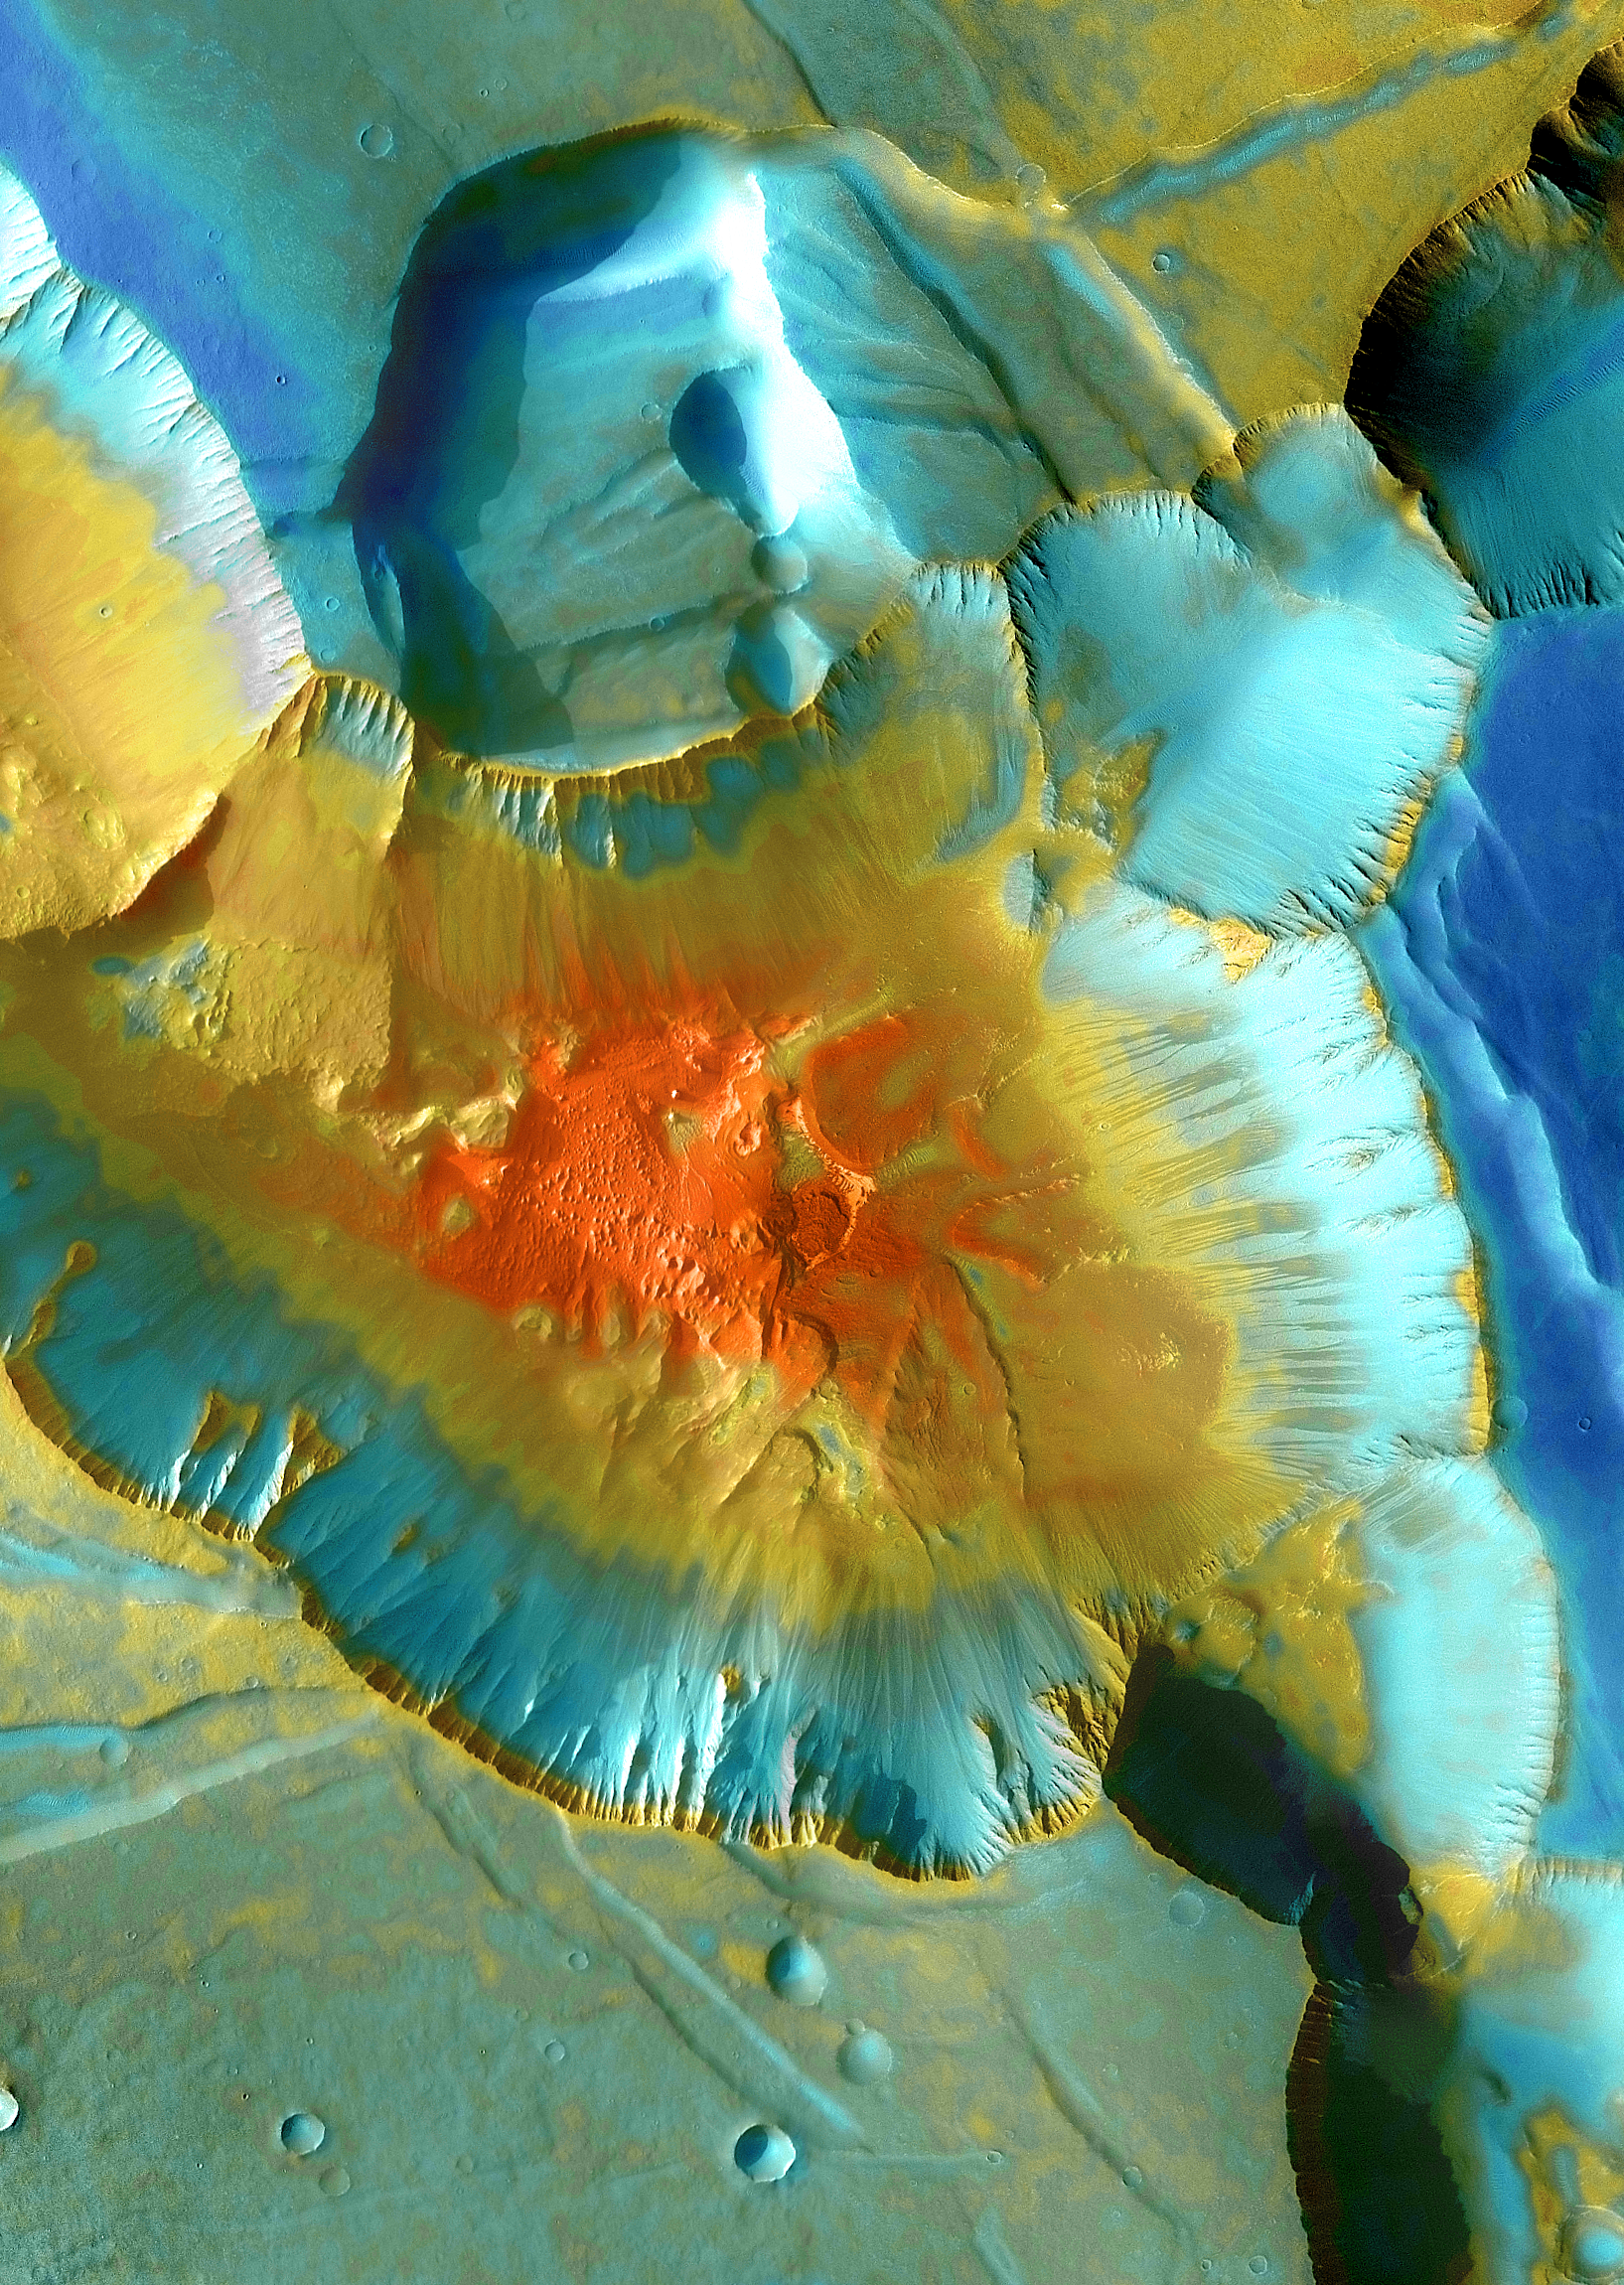
\includegraphics[scale=0.15, trim={0 5cm 0 0}, clip]{noctis_themis.png}

Noctis Labyrinthus Landslides

\url{http://themis.asu.edu/feature/6}

Location: -13.3°N, 263.4°E  
Image Size: 28x39km 1634x2300pixels

This false-color THEMIS mosaic focuses on one junction where canyons meet to form a depression 4 kilometers (13,000 feet) deep. The mosaic combines visible wavelength images made during daytime with nighttime infrared images. The nighttime view records the predawn temperature of the surface. This data can tell scientists about the nature of the materials on the ground. [...] At the foot of the slope, however, lie the traces of older, more substantial avalanches that piled up rocks and large debris. As such rockslides slow their fall and halt, they pile up ramparts that resemble the "toes" seen on the canyon floor. [...] 

In the canyon bottom lies a curious deposit whose origin is unclear. Measurements by THEMIS show this material has a temperature of –70° Celsius (–100° Fahrenheit). While this is extremely cold by Earth standards, in martian terms it's comparatively warm, especially in contrast to the dust on the canyon rim, which has a temperature of –115° C (–175° F).
 
Since the warm deposit lies where many landslide toes meet and merge, it's a good guess the material contains a lot of rocks. Yet this may not tell the complete story. In places, the deposit resembles wind-eroded features called yardangs, seen in many places on Mars.
 
Yardangs, which also occur in terrestrial desert regions, form as strong winds erode soft sediments. Typically, yardangs show as low, elongated bumps or hills that align with the prevailing wind direction.
 
Complicating the story is the fact that in the bottom of Valles Marineris and within dozens of martian craters and canyons, scientists see older material laid down in layers and now exposed by erosion. The deposits seen here partly resemble those layered sediments.
 
So is the warm, rock-rich material in the canyon bottom a mingling of landslide toes? Does it also embody wind-sculpted sediments? Or is this some unknown older material emerging as the canyon walls erode? No one can yet say - and its origin might even combine all these in some way. Stay tuned.


\section{Colonie: Landing \& Complesso Nord}

Grazie a \url{https://murray-lab.caltech.edu/CTX/V01/SceneView/MurrayLabCTXmosaic.html} è più facile farsi un'idea decente della conformazione del Noctis e del Landing.

Una possibile posizione per le varie colonie è una zona nordoccidentale del Noctis Landing. Si trova a distanza decente dal Tithonium (ancora più ripido del Noctis in molti punti), non troppo distante da Dragon Pit, relativamente a nord e vicino a una feature che potrebbe ragionevolmente essere assomigliare a una volpe (da cui i nomi dei pozzi del Complesso Nord).

\includegraphics[scale=0.15]{noctis-complesso-nord-contesto.png}

\includegraphics[scale=0.15]{noctis-complesso-nord.png}

\includegraphics[scale=0.15]{noctis-complesso-nord-annotata.png}

Altre immagini dei rendering nei files, come \texttt{noctis-landing-valley-landscape-1.png}. Sono tutte riferite alla valle di Landing (senza nome per adesso).

\includegraphics[scale=0.15]{noctis-landing-valley-landscape-10.png}

\section{Suoni}

I suoni su Marte si propagano poco per via della bassa densità e il fatto che è composa di CO2. È difficile sentire il rumore di oggetti anche relativamente vicini.

Inoltre, le onde lunghe arrivano "prima" delle onde corte, dando al suono un tipico carattere "subacqueo". L'audio della caduta di un cratere è tra i files e mostra come il suono assomiglia molto a un "blop" piuttosto che all'esplosione "asciutta, secca" che si sentirebbe sulla Terra.

\url{https://www.nasa.gov/feature/jpl/nasa-s-insight-hears-its-first-meteoroid-impacts-on-mars}

Altri audio: \url{https://mars.nasa.gov/mars2020/multimedia/audio/}



\section{Suolo vs Piante/Batteri}

"Martian soil is toxic, due to relatively high concentrations of perchlorate compounds containing chlorine. [...]

The report noted that one of the types of plant studied, Eichhornia crassipes, seemed resistant to the perchlorates and could be used to help remove the toxic salts from the environment, although the plants themselves would end up containing a high concentration of perchlorates as a result. There is evidence that some bacterial lifeforms are able to overcome perchlorates by physiological adaptations to increasing perchlorate concentrations, and some even live off them. However, the added effect of the high levels of UV reaching the surface of Mars breaks the molecular bonds, creating even more dangerous chemicals which in lab tests on Earth were shown to be more lethal to bacteria than the perchlorates alone."

Perchlorate-specific proteomic stress responses of Debaryomyces hansenii could enable microbial survival in Martian brines, Jacob Heinz, Joerg Doellinger, Deborah Maus, Andy Schneider, Peter Lasch, Hans-Peter Grossart, Dirk Schulze-Makuch


\section{Sabbia}

"The potential danger to human health of the fine Martian dust has long been recognized by NASA. A 2002 study warned about the potential threat, and a study was carried out using the most common silicates found on Mars: olivine, pyroxene and feldspar. It found that the dust reacted with small amounts of water to produce highly reactive molecules that are also produced during the mining of quartz and known to produce lung disease in miners on Earth, including cancer."

GIF di una nuvola di sabbia che si alza, Curiosity (occhio, il cielo è bianco anche qui): \url{https://photojournal.jpl.nasa.gov/catalog/PIA25361}: "This series of images from a navigation camera aboard NASA's Perseverance rover shows a gust of wind sweeping dust across the Martian plain beyond the rover's tracks on June 18, 2021 (the 117th sol, or Martian day, of the mission). The dust cloud in this GIF was estimated to be about 1.5 square miles (4 square kilometers) in size; it was the first such Martian wind-lifted dust cloud of this scale ever captured in images. This image has been enhanced in order to show maximal detail, with some color distortion."

"However, under current Martian conditions, the mass movements involved are generally much smaller than on Earth. Even the 2001 global dust storms on Mars moved only the equivalent of a very thin dust layer – about 3 µm thick if deposited with uniform thickness between 58° north and south of the equator.[42] Dust deposition at the two rover sites has proceeded at a rate of about the thickness of a grain every 100 sols."

Le tempeste di sabbia sono violente, ma non quanto sulla Terra. Avvengono di norma durante l'estate nell'emisfero australe per via della maggiore vicinanza del pianeta al sole, che causa maggiori sbalzi termici sulla superficie e quindi movimenti atmosferici più ampi. Le tempeste non raggiungono la forza di un uragano terrestre: la pressione atmosferica a livello del suolo corrisponde a un centesimo di quella terrestre e le velocità tipiche dei venti sono di circa la metà di quelle di un tipico tifone terrestre (vedi immagini per la reference).

GIF di un dust devil, Curiosity: \url{https://photojournal.jpl.nasa.gov/catalog/PIA24039} \url{https://photojournal.jpl.nasa.gov/archive/PIA24039.gif}



\includegraphics[scale=0.15, trim={25cm 0 15cm 0}, clip]{Mars_dust_storm_pillars.jpg}

\url{https://www.esa.int/About_Us/ESAC/Mars_dust_storm}

The high resolution stereo camera on board ESA’s Mars Express captured this impressive upwelling front of dust clouds – visible in the right half of the frame – near the north polar ice cap of Mars in April this year (2018).

It was one of several local small-scale dust storms that have been observed in recent months at the Red Planet, which is currently enduring a particularly intense dust storm season. A much larger storm emerged further southwest at the end of May and developed into a global, planet-encircling dust storm within several weeks.

Dust storms on Mars occur regularly during the southern summer season when the planet is closer to the Sun along its elliptical orbit. The enhanced solar illumination causes stronger temperature contrasts, with the resulting air movements more readily lifting dust particles from the surface – some of which measure up to about 0.01 mm in size.

Martian dust storms are very impressive, both visually like in this image and in terms of the intensity and duration of the rarer global events, but they are generally weaker compared to hurricanes on Earth. Mars has a much lower atmospheric pressure – less than one hundredth of Earth’s atmospheric pressure at the surface – and martian storms have less than half the typical wind speeds of hurricanes on Earth.

This colour image was created using data from the nadir channel, the field of view of which is aligned perpendicular to the surface of Mars, and the colour channels of the high-resolution stereo camera. The ground resolution is approximately 16 m/pixel and the images are centred at about 78°N/106°E.



\section{Colore del cielo}

"It is now known that during the Martian day, the sky is a butterscotch color. Around sunset and sunrise, the sky is rose in color, but in the vicinity of the setting Sun it is blue. This is the opposite of the situation on Earth. Twilight lasts a long time after the Sun has set and before it rises because of the dust high in Mars's atmosphere."

\includegraphics[scale=0.65, trim={10cm 0 10cm 0}, clip]{PIA01546_modest.jpg}

L'immagine del cielo marziano "meglio calibrata" (vedi le reference, ma dovrebbe dare una buona idea).

\url{https://photojournal.jpl.nasa.gov/catalog/PIA01546} \url{https://web.archive.org/web/20040810170442/http://humbabe.arc.nasa.gov/mgcm/faq/sky.html}

The true color of Mars based upon three filters with the sky set to aluminance of 60. The color of the Pathfinder landing site is yellowish brown with only subtle variations. These colors are identical to the measured colors of the Viking landing sites reported by Huck et al. [1977]. This image was taken near local noon on Sol 10. A description of the techniques used to generate this color image from IMP data can be found in Maki et al., 1999. Note: a calibrated output device is required accurately reproduce the correct colors.


\includegraphics[scale=0.35, trim={5cm 0 5cm 0}, clip]{Pan_Dust_Seams_2_040115174827.jpg}

\url{https://mars.nasa.gov/mer/spotlight/spirit/a12_20040128.html}

\url{https://mars.nasa.gov/mer/spotlight/spirit/images/Pan_Dust_Seams_2_040115174827.jpg}

Difference in sky color in Spirit's first panoramic images, where frames show different levels of darkness, depending on the weather when each frame was taken (light dust conditions on the left, heavy dust on the right). 


\includegraphics[scale=0.4]{Mars_dust_opacities_MER-B_Sol_1205_to_1235.jpg}

Time-lapse composite of the Martian horizon as seen by the Opportunity rover over 30 Martian days; it shows how much sunlight the July 2007 dust storms blocked; Tau of 4.7 indicates 99\% sunlight was blocked.


\includegraphics[scale=0.2]{PIA22521_sky1b.png}

\url{https://mars.nasa.gov/resources/21916/shades-of-martian-darkness/}

This series of images shows *SIMULATED* views of a darkening Martian sky blotting out the Sun from NASA’s Opportunity rover’s point of view, with the right side simulating Opportunity’s current view in the global dust storm (June 2018). The left starts with a blindingly bright mid-afternoon sky, with the sun appearing bigger because of brightness. The right shows the Sun so obscured by dust it looks like a pinprick. Each frame corresponds to a tau value, or measure of opacity: 1, 3, 5, 7, 9, 11.


\includegraphics[scale=0.35, trim={15cm 0 0 0}, clip]{PIA01547_modest.jpg}

Tramonto, Mars Pathfinder (Giugno 1999)

\url{https://photojournal.jpl.nasa.gov/catalog/PIA01547}

The brownish gray sky as it would be seen by an observer on Mars in this four-frame, true color mosaic taken on sol 24 (at approximately 1610 LST). The twin peaks can be seen on the horizon. The sky near the sun is a pale blue color. Azimuth extent is 60° and elevation extent is approximately 12°degrees. A description of the techniques used to generate this color image from IMP data can be found in Maki et al., 1999 (see full reference in Image Note). Note: a calibrated output device is required accurately reproduce the correct colors.


\includegraphics[scale=0.1]{sunset_a489_gamma_2sub_800.jpg}

Tramonto, Spirit (Maggio 2005)

\url{https://www.nasa.gov/multimedia/imagegallery/image_feature_347.html}

On May 19, 2005, NASA's Mars Exploration Rover Spirit captured this stunning view as the Sun sank below the rim of Gusev crater on Mars. This Panoramic Camera mosaic was taken around 6:07 in the evening of the rover's 489th Martian day, or sol.

Sunset and twilight images are occasionally acquired by the science team to determine how high into the atmosphere the Martian dust extends, and to look for dust or ice clouds. Other images have shown that the twilight glow remains visible, but increasingly fainter, for up to two hours before sunrise or after sunset. The long Martian twilight (compared to Earth's) is caused by sunlight scattered around to the night side of the planet by abundant high altitude dust. Similar long twilights or extra-colorful sunrises and sunsets sometimes occur on Earth when tiny dust grains that are erupted from powerful volcanoes scatter light high in the atmosphere.


\includegraphics[scale=0.4]{PIA19400_modest.jpg}

Tramonto, Curiosity (Aprile 2015)

\url{https://photojournal.jpl.nasa.gov/jpegMod/PIA19400_modest.jpg}

NASA's Curiosity Mars rover recorded this view of the sun setting at the close of the mission's 956th Martian day, or sol (April 15, 2015), from the rover's location in Gale Crater.

This was the first sunset observed in color by Curiosity. The image comes from the left-eye camera of the rover's Mast Camera (Mastcam). The color has been calibrated and white-balanced to remove camera artifacts. Mastcam sees color very similarly to what human eyes see, although it is actually a little less sensitive to blue than people are.

Dust in the Martian atmosphere has fine particles that permit blue light to penetrate the atmosphere more efficiently than longer-wavelength colors. That causes the blue colors in the mixed light coming from the sun to stay closer to sun's part of the sky, compared to the wider scattering of yellow and red colors. The effect is most pronounced near sunset, when light from the sun passes through a longer path in the atmosphere than it does at mid-day. 

Vedi anche la gif \url{https://photojournal.jpl.nasa.gov/catalog/PIA19401}

Occhio! Sembra che il cielo sia grigiastro verso lo zenith. InSight (4.5024°N 135.6234°E, Elysium Planitia) vede un cielo grigio allo zenith. Vedi \url{Color_Properties_at_the_Mars_InSight_Landing_Site.pdf} nei files per tutta l'analisi della cromaticita' del cielo (e suolo) marziani di InSight.

\includegraphics[scale=0.18, trim={0 0 40cm 0}, clip]{ess2724-fig-0013-m.jpg}

NOTA: la presenza di vapore acqueo tende a rendere il cielo piu' violaceo.

\includegraphics[scale=0.8]{PIA00915.jpg}

\url{https://photojournal.jpl.nasa.gov/catalog/PIA00915}

These clouds from Sol 15 have a new look. As water ice clouds cover the sky, the sky takes on a more bluish cast. This is because small particles (perhaps a tenth the size of the martian dust, or one-thousandth the thickness of a human hair) are bright in blue light, but almost invisible in red light. Thus, scientists expect that the ice particles in the clouds are very small. The clouds were imaged by the Imager for Mars Pathfinder (IMP).

Mars Pathfinder is the second in NASA's Discovery program of low-cost spacecraft with highly focused science goals. The Jet Propulsion Laboratory, Pasadena, CA, developed and manages the Mars Pathfinder mission for NASA's Office of Space Science, Washington, D.C. JPL is a division of the California Institute of Technology (Caltech). The Imager for Mars Pathfinder (IMP) was developed by the University of Arizona Lunar and Planetary Laboratory under contract to JPL. Peter Smith is the Principal Investigator.

Photojournal note: Sojourner spent 83 days of a planned seven-day mission exploring the Martian terrain, acquiring images, and taking chemical, atmospheric and other measurements. The final data transmission received from Pathfinder was at 10:23 UTC on September 27, 1997. Although mission managers tried to restore full communications during the following five months, the successful mission was terminated on March 10, 1998. 





\section{Acqua in atmosfera marziana}

La pressione atmosferica media di Marte sembra essere 0.6kPa, \emph{esattamente} la pressione del punto triplo dell'acqua. Esiste quindi la scarsissima probabilità di acqua liquida in superficie attorno agli 0°C, ma di norma l'acqua è gelata.

La temperatura media di Marte è -64°C, ma le variazioni sono estreme e all'equatore ci si possono aspettare temperature ben superiori allo zero, nel cui caso il ghiaccio sublima. "Martian surface temperatures vary from lows of about -110 °C to highs of up to 35 °C in equatorial summer." (Wikipedia, da \url{https://web.archive.org/web/20131102112312/http://marsrover.nasa.gov/spotlight/20070612.html})

\includegraphics[scale=0.6]{phase-diagram-water.png}

Diagramma di fase dell'acqua.

\section{Nebbia}

La nebbia probablimente può formarsi su Marte: vedi foto della nebbia del Noctis. 

La nebbia è sicuramente almeno in parte opaca, perchè appare tale dalle foto orbitali. Di conseguenza, la nebbia descritta attorno al Campo Uno è almeno possibile. Ma in che condizioni si forma e quanto è densa/persistente?

La nebbia è probabilmente resa più densa dalla presenza della sabbia, che offre un bel po' di nuclei per i cristalli di ghiaccio. Inoltre la nebbia si forma solo se l'umidità relative riesce a salire oltre il 100\% prima di raffreddarsi.

Possiamo assumere per magia che le piante marziane producano umidità al 100\% a temperature appena superiori a quelle dell'aria. In questo caso, l'aria sarebbe sempre carica di nebbia.

Essendo così fredda e rarefatta, l'atmosfera marziana richiede poca acqua per raggiungere il punto di rugiada.

Da investigare meglio.


\section{Precipitazioni: neve/brina}

Le precipitazioni sono possibili, ma tendono a non raggiungere la superficie per via della rapida sublimazione. "NASA's Phoenix Mars Lander has detected snow falling from Martian clouds. [...] A laser instrument designed to gather knowledge of how the atmosphere and surface interact on Mars has detected snow from clouds about 4 kilometers (2.5 miles) above the spacecraft's landing site. Data show the snow vaporizing before reaching the ground." \url{https://www.nasa.gov/mission_pages/phoenix/news/phoenix-20080929.html}

Nelle regioni temperate e polari (Viking) le sonde hanno trovato neve/brina di acqua e anidride carbonica.

\includegraphics[scale=0.35]{Mars_Viking_21i093.png}

Neve/Brina, Viking

\url{https://photojournal.jpl.nasa.gov/catalog/PIA00571}


This high-resolution color photo of the surface of Mars was taken by Viking Lander 2 at its Utopia Planitia landing site on May 18, 1979, and relayed to Earth by Orbiter 1 on June 7. It shows a thin coating of water ice on the rocks and soil. The time the frost appeared corresponds almost exactly with the buildup of frost one Martian year (23 Earth months) ago. Then it remained on the surface for about 100 days. Scientists believe dust particles in the atmosphere pick up bits of solid water. That combination is not heavy enough to settle to the ground. But carbon dioxide, which makes up 95 percent of the Martian atmosphere, freezes and adheres to the particles and they become heavy enough to sink. Warmed by the Sun, the surface evaporates the carbon dioxide and returns it to the atmosphere, leaving behind the water and dust. The ice seen in this picture, like that which formed one Martian year ago, is extremely thin, perhaps no more than one-thousandth of an inch thick.

\section{Nuvole}

Ci sono numerose foto di nuvole su Marte. La differenza è nel loro spessore, in quanto le nuvole marziane tendono ad essere finissime e molto difficili da vedere (vedi foto di Curiosity - occhio, quasi tutte sono in "colore terrestre").

"These clouds were captured as part of a follow-on imaging campaign to study noctilucent, or "night-shining" clouds, which started in 2021. While most Martian clouds hover no more than 37 miles (60 kilometers) above the ground and are composed of water ice, these clouds appear to be higher in elevation, where it's very cold. That suggests these clouds are made of carbon dioxide, or dry ice."

Per paragone: le nuvole terrestri di bassa quota, come i cumuli, si formano a soli 2km dalla superficie!! Persino i cirri (nuvole di alta quota) si formano a soli 3km ai poli e fino a 18km all'equatore. Siamo a neanche un terzo della quota di queste nuvole marziane.

Nuvole simili sulla Terra sono le Polar Stratospheric Clouds (PSCs) che si formano nella stratosfera polare, a circa 15-25km, e le nuvole nottilucenti, che si formano in cima alla mesosfera, ovvero a 80-85km. Queste sono ancora ben visibili. Non sono molto comuni e tendono ad assomigliare a dei cirri.

Nota che queste in foto sono tra le nuvole più basse trovate su Marte. Ce ne sono anche si mesosferiche che arrivano più in alto, anche a 100km dalla superficie.

\url{https://www.space.com/2812-mars-clouds-higher-earth.html}

"If you wanted to see these clouds from the surface of Mars, you would probably have to wait until after sunset" says Franck Montmessin, a French researcher who works with the camera team.

\textbf{This is because the clouds are very faint and can only be seen reflecting sunlight against the darkness of the night sky}. In that respect, they look similar to the mesospheric clouds, also known as noctilucent clouds on Earth, which occur about 50 miles (80 kilometers) above our planet.



\includegraphics[scale=0.27]{pia24622-curiosity_1-1041.jpg}

\url{https://photojournal.jpl.nasa.gov/catalog/PIA24622}

NASA's Curiosity Mars rover captured these clouds just after sunset on March 19, 2021, the 3,063rd Martian day, or sol, of the rover's mission. The image is made up of 21 individual images stitched together and color corrected so that the scene appears as it would to the human eye. The clouds are drifting over "Mont Mercou," a cliff face that Curiosity has been studying.

Il cielo è visibilmente troppo bianco, segno che si tratta di una delle tipiche immagini a "colore che vedresti sulla Terra".



\includegraphics[scale=0.1, trim={40cm 0 40cm 0}, clip]{PIA24662.jpg}

Iridescent clouds

\url{https://photojournal.jpl.nasa.gov/catalog/PIA24662}


NASA's Curiosity Mars rover spotted these iridescent, or "mother of pearl," clouds on March 5, 2021, the 3,048th Martian day, or sol, of the mission. Seen here are five images stitched together from a much wider panorama taken by the rover's Mast Camera, or Mastcam. The full panorama (Figure 1) was stitched together from 23 images.

Occhio: anche queste sono troppo bianche contro il cielo marziano. Dubito che a occhio si vedrebbero veramente così.



\includegraphics[scale=0.65]{PIA24661.jpg}

Drifting Clouds Over Mars' Mount Sharp, Curiosity.

\url{https://photojournal.jpl.nasa.gov/catalog/PIA24661}

This GIF shows clouds drifting over Mount Sharp on Mars, as viewed by NASA's Curiosity rover on March 19, 2021, the 3,063rd Martian day, or sol, of the mission. Each frame of the scene was stitched together from six individual images.



\includegraphics[scale=0.35]{PIA24645.png}

\includegraphics[scale=0.10]{PIA24646.jpg}

Cirri al tramonto

\url{https://photojournal.jpl.nasa.gov/catalog/PIA24645}

\url{https://photojournal.jpl.nasa.gov/catalog/PIA24646}

GIF di entrambe tra i files. Foto di Curiosity.

Using the navigation cameras on its mast, NASA's Curiosity Mars rover took these images of clouds just after sunset on March 31, 2021, the 3,075th so, or Martian day, of the mission. These noctilucent, or twilight clouds, are made of water ice; ice crystals reflect the setting sun, allowing the detail in each cloud to be seen more easily.

(stessa descrizione per entrambe le immagini)


\hfill

\includegraphics[scale=0.1, trim={20cm 0 20cm 0}, clip]{PIA25739.jpg}

Raggi di sole al tramonto, Curiosity (Marzo 2023)

\url{https://photojournal.jpl.nasa.gov/catalog/PIA25739}

NASA's Curiosity Mars rover captured these "sun rays" shining through clouds at sunset on Feb. 2, 2023, the 3,730th Martian day, or sol, of the mission. It was the first time that sun rays, also known as crepuscular rays, have been viewed so clearly on Mars. Crepuscular is taken from the Latin word for "twilight," as these rays appear near sunset or sunrise.

These clouds were captured as part of a follow-on imaging campaign to study noctilucent, or "night-shining" clouds, which started in 2021. While most Martian clouds hover no more than 37 miles (60 kilometers) above the ground and are composed of water ice, these clouds appear to be higher in elevation, where it's very cold. That suggests these clouds are made of carbon dioxide, or dry ice.

This scene made up of 28 individual images captured by the rover's Mast Camera, or Mastcam. \textbf{The images have been processed to emphasize the highlights.}


\includegraphics[scale=0.27, trim={0 15cm 0 0}, clip]{PIA25680.jpg}

InSight, fine missione

\url{https://photojournal.jpl.nasa.gov/catalog/PIA25680}

This is one of the last images ever taken by NASA's InSight Mars lander. Captured on Dec. 11, 2022, the 1,436th Martian day, or sol, of the mission, it shows InSight's seismometer on the Red Planet's surface.

Nota le nuvole "a pecorelle" sullo sfondo, un pattern notato anche in altri contesti nelle regioni polari durante la stagione delle tempeste di sabbia.

\url{https://www.esa.int/Science_Exploration/Space_Science/Mars_Express/Martian_dust_storms_churn_up_Earth-like_clouds}


\includegraphics[scale=0.35]{PIA17940_modest.jpg}

\textbf{Martian morning water ice clouds above Valles Marineris} seen by Viking Orbiter 1 (1976)

\url{https://photojournal.jpl.nasa.gov/catalog/PIA17940}

No NASA Mars orbiter has been in a position to observe morning daylight on Mars since the twin Viking orbiters of the 1970s. This image, taken by Viking Orbiter 1 on Aug. 17, 1976, shows water-ice clouds in the Valles Marineris area of equatorial Mars during local morning time. North is to the upper right, and the scene is about 600 miles (about 1,000 kilometers) across.


\includegraphics[scale=0.4, angle=180]{PIA03213_modest.jpg}

Noctis Labyrinthus, nebbia mattutina (2001) (Nord in alto a destra)

\url{https://www.esa.int/Science_Exploration/Space_Science/Mars_Express/Mars_Express_keeps_an_eye_on_curious_cloud}


As the sun rises over Noctis Labyrinthus (the labyrinth of the night), bright clouds of water ice can be observed in and around the tributary canyons of this high plateau region of Mars. This color composite image, reconstructed through violet, green, and orange filters, vividly shows the distribution of clouds against the rust colored background of this Martian desert.

The picture was reconstructed by JPL's Image Processing Laboratory using in-flight calibration data to correct the color balance.

Scientists have puzzled why the clouds cling to the canyon areas and, only in certain areas, spill over onto the plateau surface. One possibility is that water which condensed during the previous afternoon in shaded eastern facing slopes of the canyon floor is vaporized as the early morning sun falls on those same slopes. The area covered is about 10,000 square kilometers (4000 square miles), centered at 9 degrees South, 95 degrees West, and the large partial crater at lower right is Oudemans. The picture was taken on Viking Orbiter 1's 40th orbit. 





\section{Nuvole mesosferiche}

Da "Kleinböhl, A., “Clouds in the Middle Atmosphere of Mars” in: Reimuller, J. D. (ed.), Project PoSSUM –
Polar Suborbital Science in the Upper Mesosphere, Integrated Spaceflight. ã 2017." (\url{https://drive.google.com/file/d/12Fxmt85hPuFjR0GPohiMupl_Ekpp_Gdx/view}) 

Estratto dei paragrafi più interessanti sulla dinamica di formazione delle nuvole.

[...] Clouds in the martian atmosphere can be made of water ice or carbon dioxide ice. The latter do not have an equivalent on Earth as temperatures are never low enough for carbon dioxide to freeze. In addition, carbon dioxide is the main constituent of the martian atmosphere so freezing it out (either due to cloud formation or direct deposition to the surface at the winter poles) has a profound impact on the atmospheric pressure cycle and leads to significant pressure variations over the seasons.

Water ice clouds are omnipresent on Mars. Temperatures are typically suitable for the formation of ice clouds and cloud formation mainly depends on the availability of water vapor. On Earth the tropopause provides an effective cold trap for water vapor, leading to very dry conditions in the stratosphere and mesosphere. On Mars the smaller lapse rate in the atmosphere does not provide an effective cold trap for water vapor, and water ice clouds can form in the lower atmosphere as well as in the middle atmosphere. 

The most prominent cloud feature in the lower atmosphere is the aphelion cloud belt, which was already observed from Earth-based measurements. It is a band of clouds that appears in the equatorial region in the northern spring and summer season. Its typical extend is from about 10°S to 30°N in latitude and the clouds reach up to altitudes of roughly 40 km. The aphelion cloud belt is fed by water vapor coming off the north polar cap in spring and summer. The cooler global temperatures during the aphelion season cause clouds to form in the equatorial region. As the perihelion season approaches, the aphelion cloud belt starts to dissipate due to the rising global temperatures. This corresponds to northern fall. Temperatures drop in the northern high latitudes, causing condensation of water vapor in the lower atmosphere of the polar region that leads to the formation of the northern polar hood cloud. 

With an extent from the north pole down to 50°N latitude it covers not only the polar region but reaches well into the mid-latitudes. It starts forming in late northern summer around Ls=160° and dissipates again in early northern spring around Ls=20°. The southern polar region also develops a polar hood cloud in southern fall and winter. However, the southern polar water ice clouds are not nearly as dense or as extended as their counterpart in the north. They are present between about Ls=20° and Ls=180°, with a notable gap in occurrence between Ls=70° and Ls=110°. 

Like the northern polar hood, also the southern polar hood is constrained to the lower atmosphere. However, in contrast to the north, the southern polar hood cloud is shaped like an annulus, mostly covering the latitudes between 60°S and 80°S.

[...]

The most prominent feature of Figure 2 is a cloud in the equatorial region.

This is not during the season of the aphelion cloud belt. However, a temperature minimum at 30-50 km altitude between about 10°S and 40°N causes water vapor to condense and form a cloud. In addition, temperature minima at higher altitudes to the south (40°S-10°S) and to the north (40°N-60°N) lead to cloud formation. Water ice clouds in these regions are found at altitudes of 60-70 km in the middle atmosphere. This shows that at least in this season, water vapor can penetrate high enough into the atmosphere to allow the formation of water ice clouds in the middle atmosphere.

[...]
In the previous section it was shown that water ice clouds on Mars can reach mesospheric altitudes. This happens predominantly in the perihelion season (Ls=180°-360°) when the atmosphere is dustier and lower atmospheric temperatures are higher, allowing the transport of water vapor to higher altitudes of the atmosphere.

However, parts of the martian atmosphere can become cold enough to allow carbon dioxide to condense, leading to the formation of CO2 ice clouds. A feature that makes this process particularly intriguing is that CO2 is the main constituent of the martian atmosphere. In the lower atmosphere of the polar regions, temperatures in winter regularly drop to values at which CO2 condenses. The condensation of CO2 is the main driver of the seasonally varying surface pressure on Mars. In Figure 2, temperatures drop below the frost point of CO2 (~145 K at martian pressures in the lower atmosphere) in the center of the vortex close to the pole. Hence the conditions in these regions are favorable for the formation of lower atmospheric CO2 ice clouds. Due to the high abundance of CO2 in the martian atmosphere, these clouds are expected to grow to large particle sizes rather quickly, causing CO2 snowfall in the winter polar region. Observations of high clouds or detached aerosol layers in the aphelion season raised the question whether the martian mesosphere could also become cold enough to allow atmospheric CO2 to condense and form mesospheric clouds.

Observations of high clouds or detached aerosol layers in the aphelion season raised the question whether the martian mesosphere could also become cold enough to allow atmospheric CO2 to condense and form mesospheric clouds. [...] Since the 2000s, observations by instruments on several Mars orbiters including Mars Global Surveyor (MGS), Mars Express (MEx), Mars Odyssey (ODY), and the Mars Reconnaissance Orbiter (MRO) have been providing a multitude of evidence of martian middle atmospheric CO2 clouds.

[...]

One of the main drivers of temperature variations in the martian atmosphere are atmospheric tides. Tides are periodic changes in atmospheric parameters like temperature, pressure, and wind that have periods of a fraction of a solar day. They are driven by the changes of solar energy input to the Mars surface and atmosphere over the course of a day. This is in contrast to ocean tides on Earth that are driven by the gravitational pull of the moon and the sun. 

Due to the thin atmosphere on Mars, most of the solar radiation reaches the surface, where it causes strong differences in temperature between day and night. Surface temperature maxima are typically reached at local noon or slightly later, while surface temperature minima are reached in the early morning. The heat flux from the surface causes changes in pressure and temperature in the lowermost atmosphere. 

The propagation of these changes gives rise to global oscillations in atmospheric pressure and temperature, and subsequently also wind. The most prominent oscillation is the diurnal tide, which has a period of one solar day, meaning that for example temperature will exhibit one minimum as well as one maximum over the course of a day. While thermal tides also exist on Earth, their temperature perturbations typically start to become significant only at altitudes of the upper mesosphere and above. On Mars, thermal tides cause significant temperature variations throughout the atmosphere.

[...]

The right panels of Figure 7 show the occurrence of water ice clouds as observed by MCS, separated for day and night. Few water ice clouds are observed above 50 km altitude in this season. The only notable cloud occurrence in the upper middle atmosphere is observed at 60°-70°S around 70 km altitude, coincident with very low temperatures found in this region. Elsewhere water ice clouds mainly from in locations consistent with temperature minima driven by the diurnal tide. At nighttime, clouds tend to from close to the surface and around 40 km altitude in the equatorial region. At daytime the pattern reverses and clouds tend to form predominantly between 20 and 30 km altitude, where the equatorial daytime temperatures are lower than at night. 

The formation of water ice clouds is very common at temperatures found in the martian atmosphere and limited largely by the availability of water vapor. During aphelion season, water vapor in the middle atmosphere is limited by the extensive cloud formation below 40-50 km such that water ice clouds at mesospheric altitudes are rare. During perihelion season (southern spring and summer) the warmer and dustier lower atmosphere allows water vapor to be transported to higher altitudes, enabling the frequent formation of water ice clouds. Small dust particles, advected together with water vapor to mesospheric altitudes, could serve as nuclei for cloud condensation. 

The presence of clouds at altitudes of 50-70 km in perihelion season (Figure 2) indicates localized water vapor mixing ratios of tens of ppm, which would be about an order of magnitude higher than in Earth’s stratosphere and mesosphere.

[...]


\includegraphics[scale=0.4]{latitude_distribution_mesospheric_clouds.png.png}



\section{Nuvole ricorrenti}

Il meteo marziano sembra essere altamente prevedibile:  "Mars Orbiter Camera data beginning in March 1999 and covering 2.5 Martian years show that Martian weather tends to be more repeatable and hence more predictable than that of Earth. If an event occurs at a particular time of year in one year, the available data (sparse as it is) indicates that it is fairly likely to repeat the next year at nearly the same location, give or take a week."

Sembra che nel Tharsis ci siano degli ottimi esempi:
\begin{itemize}
  \item La nuvola a spirale dell'Arsia Mons: \url{https://www.jpl.nasa.gov/images/pia04294-repeated-clouds-over-arsia-mons}
  \item La nuvola allungata dell'Arsia Mons (Arsia Mons Elongated Cloud or AMEC): \url{https://www.esa.int/Science_Exploration/Space_Science/Mars_Express/Mars_Express_keeps_an_eye_on_curious_cloud}
\end{itemize}


\includegraphics[scale=0.6]{PIA04294.jpg}

La nuvola spiraliforme ricorrente dell'Arsia Mons

\url{https://www.jpl.nasa.gov/images/pia04294-repeated-clouds-over-arsia-mons}

Some parts of Mars experience weather phenomena that repeat each year at about the same time. In some regions, the repeated event may be a dust storm that appears every year, like clockwork, in such a way that we can only wish the weather were so predictable on Earth. One of the repeated weather phenomena occurs each year near the start of southern winter over Arsia Mons, which is located near 9 degrees south latitude, 121 degrees west longitude. Just before southern winter begins, sunlight warms the air on the slopes of the volcano. This air rises, bringing small amounts of dust with it. Eventually, the rising air converges over the volcano's caldera, the large, circular depression at its summit. The fine sediment blown up from the volcano's slopes coalesces into a spiraling cloud of dust that is thick enough to actually observe from orbit.

The spiral dust cloud over Arsia Mons repeats each year, but observations and computer calculations indicate it can only form during a short period of time each year. Similar spiral clouds have not been seen over the other large Tharsis volcanoes, but other types of clouds have been seen.

The spiral dust cloud over Arsia Mons can tower 15 to 30 kilometers (9 to 19 miles) above the volcano. The white and bluish areas in the images are thin clouds of water ice. In the 2005 case, more water ice was present than in the previous years at the time the pictures were obtained. For scale, the caldera of Arsia Mons is about 110 kilometers (68 miles) across, and the summit of the volcano stands about 10 kilometers (6 miles) above its surrounding plains. 


\includegraphics[scale=0.6, trim={0 10cm 0 0}, clip]{Mars_elongated_cloud_21_September_pillars.jpg}

La nuvola allungata ricorrente dell'Arsia Mons (AMEC)

\url{https://www.esa.int/Science_Exploration/Space_Science/Mars_Express/Mars_Express_keeps_an_eye_on_curious_cloud}

In spite of its location, this atmospheric feature is not linked to volcanic activity but is rather a water ice cloud driven by the influence of the volcano’s leeward slope on the air flow – something that scientists call an orographic or lee cloud – and a regular phenomenon in this region.

The cloud can be seen in this view taken on 10 October by the Visual Monitoring Camera (VMC) on Mars Express – which has imaged it hundreds of times over the past few weeks – as the white, elongated feature extending 1500 km westward of Arsia Mons. As a comparison, the cone-shaped volcano has a diameter of about 250 km [...]

Mars just experienced its northern hemisphere winter solstice on 16 October. \textbf{In the months leading up to the solstice, most cloud activity disappears over big volcanoes like Arsia Mons; its summit is covered with clouds throughout the rest of the martian year.}

However, a seasonally recurrent water ice cloud, like the one shown in this image, is known to form along the southwest flank of this volcano – it was previously observed by Mars Express and other missions in 2009, 2012 and 2015. 

The cloud’s appearance varies throughout the martian day, growing in length during local morning downwind of the volcano, almost parallel to the equator, and reaching such an impressive size that could make it visible even to telescopes on Earth.

The formation of water ice clouds is sensitive to the amount of dust present in the atmosphere. These images, obtained after the major dust storm that engulfed the entire planet in June and July, will provide important information on the effect of dust on the cloud development and on its variability throughout the year.

The elongated cloud hovering near Arsia Mons this year was also observed with the visible and near-infrared mapping spectrometer, OMEGA, and the High Resolution Stereo Camera (HRSC) on Mars Express, providing scientists with a variety of different data to study this phenomenon.



\chapter{Phobos \& Deimos}

\section{Dimensioni relative}

\includegraphics[scale=0.5]{PIA17351.jpg}
\includegraphics[scale=0.2]{dimensione_phobos_sole.png}

\url{https://photojournal.jpl.nasa.gov/catalog/PIA17351}

This illustration provides a comparison for how big the moons of Mars appear to be, as seen from the surface of Mars, in relation to the size that Earth's moon appears to be when seen from the surface of Earth. Earth's moon actually has a diameter more than 100 times greater than the larger Martian moon, Phobos. However, the Martian moons orbit much closer to their planet than the distance between Earth and Earth's moon.

Deimos, at far left, and Phobos, beside it, are shown together as they actually were photographed by the Mast Camera (Mastcam) NASA's Mars rover Curiosity on Aug. 1, 2013. The images are oriented so that north is up. The size-comparison image of Earth's moon, on the right, is also oriented with north up.

Deimos has a diameter of 7.5 miles (12 kilometers) and was 12,800 miles (20,500 kilometers) from the rover at the time of the image. Phobos has a diameter 14 miles (22 kilometers) and was 3,900 miles (6,240 kilometers) from the rover at the time of the image. Earth's moon has a diameter of 2,159 miles (3,474 kilometers) and is typically about 238,000 miles (380,000 kilometers) from an observer on Earth. 




\includegraphics[scale=0.5]{PIA13737.png}

\url{https://photojournal.jpl.nasa.gov/catalog/PIA13737} (video tra i files)

The larger of the two moons of Mars, Phobos, transits (passes in front of) the sun in this approximately true-speed movie simulation using images from the panoramic camera (Pancam) on NASA's Mars Exploration Rover Opportunity taken on the rover's 2,415th Martian day, or sol (Nov. 9, 2010). The movie includes images that have been calibrated and enhanced, plus simulated frames used to smooth the action.

Images of solar transits of Phobos and the other Mars moon, Deimos, taken over many years by Mars rovers aid in studies of slight changes in the moons' orbits.

This movie is based on 10 individual photos taken through the Pancam's special solar filter every four seconds during the transit, which lasted about 32 seconds. The images were gradually blended together to create a simulated near-real-speed animation of the event. The moviemakers supplemented those images with sky color information from a pair of images taken right after the transit through two regular imaging filters: one centered on a wavelength of 440 nanometers (blue) and the other on 750 nanometers (near infrared).

\textbf{The silhouette of Phobos looks smaller than in some other Mars rover transit images (for example, PIA05554) because when Phobos is near the horizon it is more than 30 percent farther from the camera's location than when it is straight overhead.}

\section{Albedo e luminosità}

Phobos sembra essere piuttosto scura, ma ha un albedo simile a quello lunare. Considerata anche la dimensione (luna: 0.5°, phobos: 0.2°), Phobos piena dovrebbe illuminare come una mezzaluna, considerando il cielo limpido. 

\hfill

\includegraphics[scale=0.1, trim={50cm 0 50cm 0}, clip, angle=90]{H7982_0000_ND2_phobos_on_limb.jpg}

Foto qualunque di Phobos sull'orizzonte marziano, Mars Express. Così poco rilevante che l'ho trovata su un forum da un tizio che l'ha scaricata dalla cartella FTP di Mars Express (HRSC, High Resolution Stereo Camera). 

\url{http://www.unmannedspaceflight.com/index.php?s=50e274fb401c38cab101ba75a3e1c9cf&showtopic=480&st=195&p=167059&#entry167059}


La foto "sorella" verrà poi croppata e pubblicata da APOD (\url{https://apod.nasa.gov/apod/ap101201.html})

Data del post:  Nov 25 2010, 09:26 PM. Probabile che le foto siano state caricate poco prima, quindi scattate nella seconda metà di Novembre 2010. \url{http://www.unmannedspaceflight.com/index.php?s=50e274fb401c38cab101ba75a3e1c9cf&showtopic=480&st=195&p=167059&#entry167059}

Trovata anche su un mirror degli archivi FTP dell'ESA (HRSC, orbita 7982):
\url{https://archives.esac.esa.int/psa/ftp/MARS-EXPRESS/HRSC/MEX-M-HRSC-3-RDR-EXT3-V4.0/BROWSE/7982/H7982_0000_ND3.JPG}

Colorizzata da me per la copertina de "Lo spettro", vedi cartella dedicata.



\section{Ombra di Phobos \& Eclissi solari}

Phobos orbita molto velocemente e in senso opposto al sole. Inoltre lo eclissa regolarmente.

L'ombra di Phobos è quindi visibile abbastanza di frequente da Phobos stessa sulla superficie marziana, vedi foto.

\url{https://en.wikipedia.org/wiki/Transit_of_Phobos_from_Mars}

"A transit of Phobos from Mars usually lasts only thirty seconds or so, due to the moon's very rapid orbital period of about 7.6 hours.

Because Phobos orbits close to Mars and in line with its equator, transits of Phobos occur somewhere on Mars on most days of the Martian year. Its orbital inclination is 1.08°, so the latitude of its shadow projected onto the Martian surface shows a seasonal variation, moving from 70.4°S to 70.4°N and back again over the course of a Martian year. Phobos is so close to Mars that it is not visible south of 70.4°S or north of 70.4°N; for some days in the year, its shadow misses the surface entirely and falls north or south of Mars.

At any given geographical location on the surface of Mars, there are two intervals in a Martian year when the shadow of Phobos or Deimos is passing through its latitude. During each such interval, about half a dozen transits of Phobos can be seen by observers at that geographical location (compared to zero or one transits of Deimos). Transits of Phobos happen during Martian autumn and winter in the respective hemisphere; close to the equator they happen around the March and September equinoxes, while farther from the equator they happen closer to the winter solstice.

Observers at high latitudes (but less than 70.4°) will see a noticeably smaller angular diameter for Phobos because they are considerably farther away from it than observers at Mars's equator. As a result, transits of Phobos for such observers will cover less of the Sun's disk. Because it orbits so close to Mars, Phobos cannot be seen north of 70.4°N or south of 70.4°S; observers at such latitudes will obviously not see transits, either."

Riguardo alla possibilità di vedere l'ombra di Phobos dallo spazio: 

"Viewed from orbit, the penumbral shadow of Phobos can be seen to move rapidly over the Martian surface. This shadow on the Martian surface has been photographed on many occasions by Mars Global Surveyor. 

In the 1970s, the Viking 1 Lander and Orbiter photographed the shadow as well. The Lander detected the penumbral shadow of Phobos passing across it. This was detected only as a slight dimming of the ambient light; the Viking 1 Lander camera did not image the Sun. The shadow took about 20 seconds to pass over the Lander, moving at about 2 km/s. The shadow was simultaneously imaged from the Viking 1 Orbiter, which permitted locating the position of the lander in the orbiter pictures."

Aggiungo anche una GIF del transito sull'intero disco (\url{https://www.planetary.org/space-images/phobos-shadow-transits-mars}, \texttt{20130820\_mex\_vmc\_20100131\_anim\_phobos\_transit.gif}), con la seguente descrizione: 

"Phobos' shadow transits Mars In a six-frame animation spanning 15 minutes over January 30-31, 2010, the Mars Express Visual Monitoring Camera observed Phobos' shadow transiting Mars. \textbf{It is late autumn in Mars' southern hemisphere, so the shadow of Phobos (which orbits exactly along Mars' equatorial plane) falls on Mars' high southern latitudes}. Mars Express is looking down nearly onto Mars' south pole, which is in winter darkness; the bright splat at the center of the animation is the Argyre impact basin, with the crater Galle located on its rim. Phobos' shadow crosses northern Argyre and proceeds across Noachis terra. This is the first time that VMC wasknown to have imaged Phobos' shadow"

Mooolto piccola, a stento visibile nella GIF. Almeno da l'idea della velocità del transito.

Un'altra gif colorizzata e ottenuta dai dati di Viking1 è \url{phobos_shadow_viking1_colorized.mp4}, nelle note. Link di Youtube: \url{https://www.youtube.com/watch?v=ry3HYHpnURI} Trovata qui: \url{https://www.planetary.org/articles/2830} 

Dalla descrizione: "Viking 1 observes a dust storm and Phobos’ shadow On September 28, 1977, Viking Orbiter 1 observed a dust storm over the site where it had dropped its lander, a little more than a year previously. As Viking 1 orbiter watched, the shadow of Mars' inner moon Phobos passed over the cloud tops. The sequence of images has been artificially colorized and is \textbf{displayed at a speed ten times that of real time}. (Viking images f467a31 - f467a69)"

Qui si vede molto bene quanto difficile sia scorgere l'ombra di Phobos. Forse è meglio considerarla non visibile?


\includegraphics[scale=0.6]{Phobos_shadow.jpg}

Ombra di Phobos su Marte, MSSS Mars Global Surveyor, 1999

(Wikimedia, non trovo il link originale: \url{https://en.wikipedia.org/wiki/File:Phobos_shadow.jpg} Parte di \url{https://asimov.msss.com/moc_gallery/ab1_m04/images/M0403241.html} e \url{https://asimov.msss.com/moc_gallery/ab1_m04/images/M0403242.html}) 

The penumbral shadow of Phobos is visible on the landscape of Mars, as photographed by the Mars Global Surveyor. The center of the shadow was at approximately 10.9°N 49.2°W (Map of area Map zoom) at 04:00:33.3 UTC Earth time.

The image shows western Xanthe Terra on August 26 1999 at about 2:41 p.m. local solar time on Mars. The image covers an area about 250 kilometers across and is illuminated from the left. The dark spots on the crater floors are probably dark sand dunes. None of the craters pictured currently have names. Nanedi Valles is the meandering valley at the bottom right. The picture covers about 7°–15°N vertically and 52°–48°W horizontally. The vertical orientation of the image is 3.01° to the west of north; a north-pointing arrow superimposed on the image would point slightly to the right.

To determine the time of the shadow, we can look up the original image files at M04-03241 (red) \url{https://asimov.msss.com/moc_gallery/ab1_m04/nonmaps/M0403241.gif} and M04-03242 (blue) \url{https://asimov.msss.com/moc_gallery/ab1_m04/nonmaps/M0403242.gif}. The "image start time" was 03:26:13.01 UTC, the "line integration time" is 80.4800 milliseconds, and the "downtrack summing" factor is 4. Since the shadow is centered at 6400 pixels from the bottom of the original 10800-pixel-high image (Mars Global Surveyor had a south-to-north sun-synchronous orbit), we add (6400 * 0.08048 * 4) = 2060.3 seconds = 34 minutes 20.3 seconds to get a time of 04:00:33.3 UTC for the center of the shadow. 

\begin{verbatim}
Ancillary data for MOC wide-angle image M04-03241
Acquisition parameters

     Image ID (picno): M04-03241
     Image start time: 1999-08-26T03:26:13.01 SCET
         Image  width:    256      pixels
         Image height:  10800      pixels
Line integration time:     80.4800 millisec
   Pixel aspect ratio:      1.03
   Crosstrack summing:      4
    Downtrack summing:      4
     Compression type: MOC-NONE
            Gain mode:     3A (hexadecimal)
          Offset mode:      5 (decimal)

	Derived values

Longitude of image center:     47.47°W
Latitude  of image center:      5.68°S
       Scaled pixel width:    961.72   meters
      Scaled image  width:    258.01   km
      Scaled image height:  10556.75   km
     Solar longitude (Ls):    194.55°
    Local True Solar Time:     14.25   decimal hours
           Emission angle:      3.54°
          Incidence angle:     40.67°
              Phase angle:     37.14°
            North azimuth:     93.01°
              Sun azimuth:      0.17°
      Spacecraft altitude:    380.63   km
           Slant distance:    381.29   km
\end{verbatim}


Il raggio di Marte è circa 3300km, quindi diametro di 6600km. L'ombra di Phobos, a giudicare dalle immagini e dai dati, è ampia circa 90px * 1000m = 9km, mooooolto piccola rispetto al disco. D'altra parte, Phobos orbita a quota molto bassa. Quanto ampa risulta essere l'ombra a quella distanza?

Periapsi di Phobos: cca 9000km

Apparent size  = diametro/distanza * 3438 arcominuti = 9km / 9000km * 3438 $\simeq$ 3' (dimensione dell'ombra vista dall'orbita di Phobos). Per paragone, il Sole sulla Terra è ampio 32', mentre Venere o la ISS sono circa a 1'.

Quindi visibile, ma molto piccola. Probabilmente si vede abbastanza bene se si presta attenzione, perchè si muove, anche se è solo penumbrale.

\section{Eclissi "lunari"}

Al contrario, le eclissi lunari (ombra di Marte su Phobos) sembrano più complicate. Secondo questo articolo veramente arcaico (che parla di marziani!! :D) \url{https://ui.adsabs.harvard.edu/abs/1923PPCAS...8...10C/abstract} (è nei files, 'eclipses\_on\_mars\_1923.pdf') il fenomeno avviene solo per un terzo dell'anno e con lunghezze tra i pochi minuti e la mezz'ora. Per il momento mi fido dato che il resto sembra sufficientemente accurato (eccetto per il diametro di Phobos che, secondo l'articolo, è sufficiente a causare eclissi solari totali, il che non è vero).

\section{Dimensione di Marte da Phobos}

Lo stesso calcolo (Apparent size  = diametro/distanza * 3438 arcominuti) dice che il disco di Marte è di 2521', ovvero 42°. 

Nota che il campo visivo umano è di 210° orizzontali e 150° verticali, per cui il disco di Marte si riesce a vedere per intero, anche considerando solo la visione binoculare che è 120°H-60°V.

Per esempio, immagine di Marte visto da Phobos, apertura immagine 90°:

\includegraphics[scale=0.4]{mars-from-phobos-90deg-angle.jpeg}

Ottenuta dal simulatore della NASA: \url{https://space.jpl.nasa.gov/cgi-bin/wspace?tbody=499&vbody=401&month=4&day=28&year=2023&hour=00&minute=00&fovmul=1&rfov=90&bfov=30&showac=1}




\chapter{Europa}

\section{Quadrangoli e nomenclature}
Quadrangoli di Europa (Je): 
\begin{itemize}
  \item \url{https://upload.wikimedia.org/wikipedia/commons/8/82/Europa_USGS_map.jpg}
  \item \url{https://solarviews.com/eng/eurmap.htm}
  \item \url{https://www.researchgate.net/publication/234039235_Geologic_mapping_of_Europa}
\end{itemize}

\url{https://en.wikipedia.org/wiki/Epona}

Emain Ablach: \url{https://en.wikipedia.org/wiki/Emain_Ablach}
  
\section{Giove nel cielo di Europa}

Esempio dal simulatore della NASA \url{https://space.jpl.nasa.gov/}, apertura 90°, prossimo a un eclisse solare:

\includegraphics*[scale=0.4]{jupiter-from-europa-90deg-angle-about-to-eclipse.jpeg}

Giove pieno (o quasi):

\includegraphics*[scale=0.4]{jupiter-from-europa-90deg-angle-full.jpeg}

Europa è tidally locked con Giove, per cui Giove appare fisso in cielo e si vede solo dall'emisfero rivolto verso di esso. Ma: da dove lo si vede??

Il sub-jovian point sembra essere circa nel pressi del cratere Callanish (studiando a occhio il rendering della Nasa :D \url{https://solarsystem.nasa.gov/planets/jupiter/overview/}). 

Dal Conamara Chaos (60° più a est, Je-09 Belus Linea), Giove dovrebbe apparire basso sull'orizzonte occidentale.

Dato che Giove è ampio 13.4° quando visto da Europa, dovrebbe essere ancora interamente visibile in cielo: 90 - (60+(13/2)) $>$ 0

Apparent size / 3438 arcminutes =  Diameter (km) / Distance (km)

Jupiter has a diameter of 142,000 km. Europa has a diameter of 2960 km. Distance varies between 604,000 and 592,000 km

Un altro indizio: immagine del trailing emisphere: \url{https://www.planetary.org/space-images/europa_g2_stryk} 

Trailing emisphere: As Europa moves in its orbit around Jupiter, the trailing hemisphere is the portion which is always on the moon's backside opposite to its direction of motion.

Quindi il sub-jovian meridian dovrebbe essere sul perimetro occidentale del trailing emisphere

Dall'immagine sembra che il Callanish sia ancora nel pieno del trailing. Giove dovrebbe essere visibile da qualunque punto nella metà occidentale del trailing emisphere, ma il Conamara è già nella metà est!

Meglio usare il Callanish stesso, dato che da lì Giove è "sicuramente" visibile.

Callanish sta in Je-10 Callanish (non c'è praticamente nessun'altra feature sulla mappa con cui dare un nome al quadrante :( )

"Europa orbits Jupiter in just over three and a half days, with an orbital radius of about 670,900 km. With an orbital eccentricity of only 0.009, the orbit itself is nearly circular, and the orbital inclination relative to Jupiter's equatorial plane is small, at 0.470°."

"Because of this, there is a sub-Jovian point on Europa's surface, from which Jupiter would appear to hang directly overhead. Europa's prime meridian is a line passing through this point." \url{https://en.wikipedia.org/wiki/Europa_(moon)#Orbit_and_rotation}. E sulla mappa si vede benissimo dov'è il meridiano zero: poco a destra delle Callanish. In sostanza la posizione di Giove in cielo corrisponde \textbf{sempre} all'equivalente posizione sul terreno: sul meridiano zero a latitudine zero, Giove è allo zenith.

Quindi dalla Callanish Giove sta 17-18° dallo zenith verso nord e 25° dallo zenith verso ovest. Molto alto a nordovest insomma.

Simile la situazione attorno alla Kennet, ma più basso: -40 dallo zenith a nord e a ovest. Giove è ampio 13 gradi, per cui è ben alto sull'orizzonte.

FASI DI GIOVE: siccome Europa è tidally locked con Giove, le fasi sono opposte: a mezzogiorno Giove è nuovo (e c'è un'eclisse, necessariamente), mentre di notte Giove diventa pieno. Tener conto che la giornata/mese dura 3.5 giorni su Europa, circa 84h.

Foto di Giove usata per l'immagine in copertina: \url{https://www.planetary.org/space-images/jupiter_crescent_19970903} (Galileo, September 3, 1997)
  

\includegraphics[scale=0.35]{europa-trailing-emisphere-galileo-1996.jpg}

Trailing emisphere of Europa, Galileo, 1996. Nord in alto. Falso colore. 

Il cratere a destra è il Pwyll, quello a sinistra il Callanish, la macchia appena sotto la X il Conamara Chaos.
Il Mannanán, dove si trova la Colonia Emain, non è visibile, anche se dovrebbe essere nell'immagine sull'orlo orientale (spostato sul Rhiannon, al polo sud, dove il problema si pone meno).



\section{Radioattività del suolo}

Secondo questa mappa della radioattività di Europa \url{https://europa.nasa.gov/news/17/radiation-maps-of-europa-key-to-future-missions/}, l'equatore è parecchio più radioattivo dei poli. Quindi è meglio spostare la base AT dal Mannanán a un cratere polare, per esempio Rhiannon

Europa è fosforescente al buio per via delle radiazioni: \url{https://www.nasa.gov/feature/jpl/europa-glows-radiation-does-a-bright-number-on-jupiters-moon}

\url{https://en.wikipedia.org/wiki/Penitente_(snow_formation)}

\hfill 

\includegraphics[scale=0.4]{europa-radiation-map.png}

Mappa della radioattività superficiale di Europa. (\url{https://europa.nasa.gov/news/17/radiation-maps-of-europa-key-to-future-missions/}).

Questa fantastica mappa finalmente chiarisce che l'intuizione sopra è corretta e il Callanish sta vicino al sub-jovian meridian. Zona rosa: zona con più alta radioattività rispetto al resto della superficie.



\section{Lineae e criovulcani}

"Geysers": \url{https://www.nasa.gov/content/goddard/hubble-europa-water-vapor}

Le lineae sono sottili! Dalle foto sembrano essere large circa 2km, quindi mezz'ora di cammino, dieci-quindici minuti di corsa terrestre, quindi ancora meno su Europa immaginando che la "corsa" in bassa gravità sia più efficiente e veloce. 

Prove: \texttt{minos-linea-228meters-pixel.png} (da \url{https://www.planetary.org/space-images/lineae-on-europa}), l'immagine rappresenta lineae spesse come Minos e Udaeus, sono 228 metri per pixel, eppure lo spessore è di appena 16-20px, il che sigifica 20x200 = 4000, 4km nel punto più largo in assoluto. Comunque meno di un'ora anche andando al passo. E Kennet sembra più piccola.


\includegraphics{minos-linea-228meters-px-crop.png}

Dimensione delle Lineae: crop della Minos, una delle più larghe, con le misure. \texttt{minos-linea-228meters-pixel.png} (da \url{https://www.planetary.org/space-images/lineae-on-europa})
  
  




\chapter{Altro: fisica, chimica, medicina, ...}


\section{Delta-v del Sistema Solare}

\includegraphics[scale=0.2]{Solar-system-delta-v-map.png}

\section{Sistema di coordinate nel sistema solare}

Il sistema utilizzato su scala interplanetaria (ovvero per specificare la posizione di vari pianeti-navi-astaroidi rispetto al Sole) è il sistema eclittico eliocentrico \url{https://en.wikipedia.org/wiki/Ecliptic_coordinate_system}.

Sistemi eclittici si possono anche centrare su un pianeta specifico, per esempio come si fa con la Terra.

Le coordinate (sferiche) vengono chiamate:

\begin{itemize}

  \item Eliocentrico: longitudine l, latitudine b, distanza r
  \item Geocentrico: longitudine $\lambda$, latitudine $\beta$, distanza $\Delta$

\end{itemize}

Utilizzerò la convenzione geocentrica per tutti i sistemi centrati su un nucleo planetario.


\section{Parametri orbitali}

Simulatore di orbite (solo eliocentriche): \url{https://ssd.jpl.nasa.gov/tools/orbit_diagram.html}

Simulatore che supporta Saturno: \url{https://gravitysimulator.org/solar-system/saturn-and-its-rings-and-major-moons}

L'orbita prevista dell'Hoyle potrebbe essere una Molniya, quindi (per la Terra):
\begin{itemize}
\item Argument of perigee: 270°
\item Inclination: 63.4°
\item Period: 718 minutes (questo è probabilmente diverso per Saturno)
\item Eccentricity: 0.74
\item Semi-major axis: 26,600 km (questo è ovviamente diverso per Saturno)
\end{itemize}

Screenshot di un esempio nei files: \texttt{orbit-designer-ezample-molniya.png}

\section{Distanza dell'orizzonte}

"Distance to the true horizon from an observer close to the Earth's surface is about $d \simeq \sqrt{2 h R}$  where h is height above sea level and R is the Earth radius. For instance, in standard atmospheric conditions, for an observer with eye level above sea level by 1.70 metres (5 ft 7 in), the horizon [on Earth] is at a distance of about 5 kilometres."

Marte ha un raggio di circa 3300km, quindi $d \simeq \sqrt{2*1.7m*3300000m} \simeq 3.3$km

Europa ha un raggio di circa 1561km, quindi $d \simeq \sqrt{2*1.7m*1561000m} \simeq 2.3$km

\section{Deprivazione del sonno}

Un resoconto che rende l'idea molto meglio delle varie descrizioni mediche: \url{https://mattlakeman.org/2020/05/11/96-hour-no-sleep-challenge/}

Sembra che:
\begin{itemize}
\item a 15-16h se ne sentono i primi effetti (sonno e stanchezza).
\item 24h sono ancora tollerabili e si riesce, con un certo sforzo, a stare svegli e a fare qualcosa.
\item a 36h gli effetti pericolosi diventano incontrollabili (nebbia mentale, fatica intensa, sonno intenso, livello di attenzione ridicolo, microsleep etc)
\item Attività "intense" (nel caso del post, videogames e interazioni con altre persone) combattono gli effetti in modo molto forte.
\end{itemize}

Altre info più "tecniche" da Wikipedia:

The U.S. military has studied fatigue countermeasures. An Air Force report states: "Each individual nap should be long enough to provide at least 45 continuous minutes of sleep, although longer naps (2 hours) are better. In general, the shorter each individual nap is, the more frequent the naps should be (the objective remains to acquire a daily total of 8 hours of sleep)."

Similarly, the Canadian Marine pilots in their trainer's handbook report that: "Under extreme circumstances where sleep cannot be achieved continuously, research on napping shows that 10- to 20-minute naps at regular intervals during the day can help relieve some of the sleep deprivation and thus maintain ... performance for several days. However, researchers caution that levels of performance achieved using ultrashort sleep (short naps) to temporarily replace normal sleep are always well below that achieved when fully rested."

The Italian Air Force (Aeronautica Militare Italiana) also conducted experiments for their pilots. In schedules involving night shifts and fragmentation of duty periods through the entire day, a sort of polyphasic sleeping schedule was studied. Subjects were to perform two hours of activity followed by four hours of rest (sleep allowed), this was repeated four times throughout the 24-hour day. Subjects adopted a schedule of sleeping only during the final three rest periods in linearly increasing duration. The AMI published findings that "total sleep time was substantially reduced as compared to the usual 7–8 hour monophasic nocturnal sleep" while "maintaining good levels of vigilance as shown by the virtual absence of EEG microsleeps." EEG microsleeps are measurable and usually unnoticeable bursts of sleep in the brain while a subject appears to be awake. Nocturnal sleepers who sleep poorly may be heavily bombarded with microsleeps during waking hours, limiting focus and attention.

\section{Miniere}

Un esempio interessante è la Miniera Kidd, in Canada, tra le più profonde al mondo. La pianta non è ovvia e segue la vena di metalli con tre pozzi, il più profondo dei quali inizia già a grande profondità.

Un'altra è LaRonde, una miniera d'oro canadese, la quale offre pure un modello 3D della miniera: \url{https://www.youtube.com/watch?v=8ubtBRMc9cQ}. La compagnia offre rendering 3D di molte altre miniere sotterranee: \url{https://youtube.com/playlist?list=PLtwVkIGRIcKqJfrQelCqCXnrtk5_SUDCF}

\includegraphics[scale=0.4]{Underground_mine_3D_model.jpg}
Esempio generico.

\includegraphics[scale=0.4]{kidd_creek_mine_layout.jpg}

Kidd Creek. Questa è la parte cruciale: dei pozzi verticali da cui partono tunnel orizzontali ogni 100-150m di profondità nella direzione dei depositi, che poi vengono scavati fino a svuotarli. Delle rampe collegano i vari livelli per permettere ai mezzi di muoversi, ma i minerali escono dai pozzi. Il crusher credo serva a polverizzare i minerali per ottimizzare il trasporto: in pratica i minerali vengono prima mandati giù in fondo al pozzo, da cui poi risalgono.

\includegraphics[scale=0.5]{kidd_creek_mine_layout_2.jpg}

\includegraphics[scale=0.5]{kidd_creek_mine_layout_6000ft_level.jpg}

\includegraphics[scale=0.7]{kidd_creek_mine_surface.jpg}

\includegraphics[scale=0.5]{kidd_creek_mine_internal_control_system_interface.jpg}



\section{Cobalto-60}
Co60 half life: 5.2713 years \url{https://en.wikipedia.org/wiki/Cobalt-60}

Co60 is normally used for medical devices sterilization due to high penetration gamma rays production during decay: \url{http://www-naweb.iaea.org/napc/iachem/Brochgammairradd.pdf}

Il cobalto non si bioaccumula: l'eccesso viene espulso via urina e feci nell'arco di ore-giorni. 
\begin{itemize}
  \item Attenzione: Co58/Co59, non Co60! Sarà uguale?
  \item Kirchgessner M., Reuber S., Kreuzer M. (1994). Endogenous excretion and true absorption of cobalt as affected by the oral supply of cobalt. Biol. Trace Elem. Res. 41, 175–189.
  \item \url{https://link.springer.com/article/10.1007/BF02917227}
  \item \url{https://pubmed.ncbi.nlm.nih.gov/7946905/}
\end{itemize}


% Fine

\end{document}